\chapter{Weakly-supervised Approach}
\label{ch:weakley_supervised}
Unsupervised methods, consider a human fall as an event that deviate from normality and they are based on one-class classifiers. The main advantage of an unsupervised methods for fall detection is that it can works without knowing any examples related the the class of interest, i.e. the human fall. As aforementioned, this should be the perfect way to go in an application like this, where what we are interested in is very difficult to retrieve or we only have very few data available, but the principal weakness of an unsupervised system is that certain events deviate from normality as the human fall (e.g., the fall of an object), thus they may produce false alarms.
Moreover, in some applications, like the fall detection task, it can be difficult to obtain
strong supervision information due to the high cost of the data-labeling process. Thus, it is desirable for machine-learning techniques to be able to work with weak supervision.
The weak-supervision is a generic term that include different kind of techniques \cite{zhou2017brief}:
\begin{itemize}
	\item ``incomplete supervision'' where the labels are available only for a small subset of training;	
	\item ``inexact supervision'' where only coarse labels with respect to the samples are provided
	\item ``inaccurate supervision'' where the labels are not always correct.
\end{itemize}

In this Chapter, methods belogning to the first an second category are described: in \secref{sec:user_aided_cin} a semi-supervised OCSVM method, that is a subcategory of the ``incomplete supervision'' problem \cite{zhou2017brief}, is exposed. Instead, in \secref{sec:siamese_few_shot} present an approach based on Siamese neural network for one-shot learning in a ``inexact supervision'' context. Both of them, has been assessed with samples related to R0 room of the employed dataset \secref{sec:dataset}. An extension of the Siamese approach is presented in \secref{sec:siamese_few_shot} where the entire dataset described in \secref{sec:dataset} has been used.




\section{A Combined One-Class SVM and Template Matching Approach for User-Aided Human Fall Detection}
\label{sec:user_aided_cin}

The approach proposed here, is the extension of the one presented in \secref{sec:ocsvm_approach} thus, consists of a combined One-Class Support Vector Machine (OCSVM) based method and template-matching classifier that operate in cascade. The template-matching classifier operates in a user-aided supervised manner and it is employed to reduce such errors by using a set of templates that represent these events. Templates are identified by the user that marks the occurrence of a false positive instead of a true human fall event. 
As shown in the previous section, ``unsupervised methods'' are able to overcome the need of manual tuning of ``analytical methods'' and the necessity of a large labelled dataset of ``supervised methods''. In ``unsupervised methods'', falls are discriminated from non-falls based on a model of ``normality'' constructed from a large amount of non-fall events. However, certain events differ from the ``normality'' as human falls, and they may induce the classifier to produce false alarms. As an example, \figref{fig:time_ha} and \figref{fig:spec_ha} show respectively the waveform and the spectrogram of a segment of ``normal'' human activity (footsteps and speech) \figref{fig:time_hf} and \figref{fig:spec_hf} show the waveform and the spectrogram of a segment of human fall, and \figref{fig:time_bf} and \figref{fig:spec_bf} the waveform and the spectrogram of a book fall. The figures show clearly that both falls signals differ significantly from the human activity one, thus a classifier may be induced to consider the fall of a book as the fall of a person.

\begin{figure}[htbp!]
	\centering
	\begin{subfigure}[ht]{0.5\columnwidth}
		\centering
		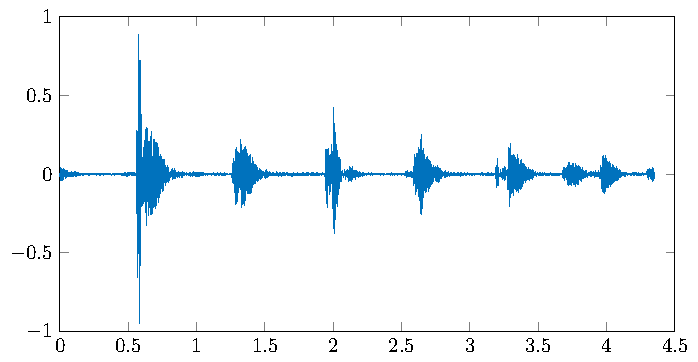
\includegraphics[width=0.9\textwidth]{img/cin/ha_time_.pdf}
		\caption{Normal human activity signal in the time domain.}\label{fig:time_ha}
	\end{subfigure}%
	\begin{subfigure}[ht]{0.5\columnwidth}
		\centering
		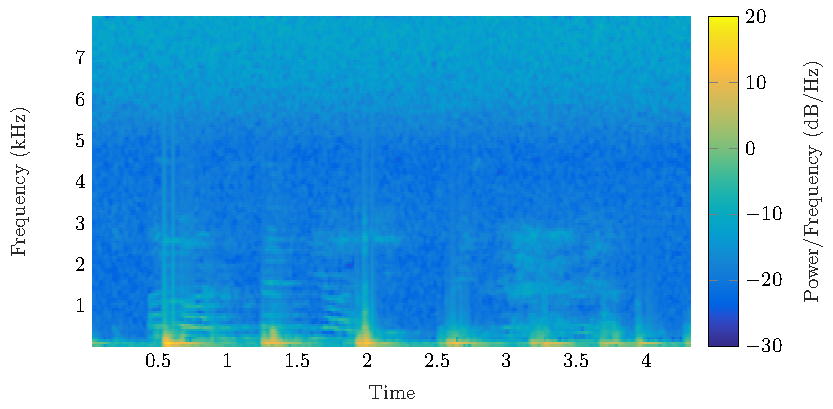
\includegraphics[width=\textwidth]{img/cin/ha_freq_.pdf}
		\caption{Normal human activity signal in the frequency domain.}\label{fig:spec_ha}
	\end{subfigure}
	
	\begin{subfigure}[ht]{0.5\columnwidth}
		\centering
		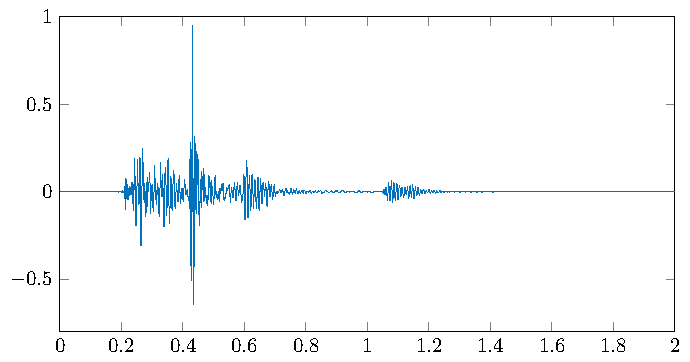
\includegraphics[width=0.9\textwidth]{img/cin/rndy_time_.pdf}
		\caption{Human fall signal in the time domain.}\label{fig:time_hf}
	\end{subfigure}%
	\begin{subfigure}[ht]{0.5\columnwidth}
		\centering
		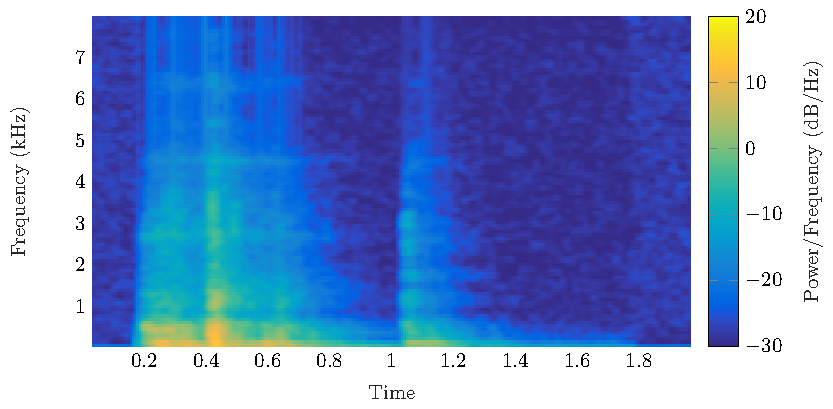
\includegraphics[width=\textwidth]{img/cin/rndy_freq_.pdf}
		\caption{Human fall signal in the frequency domain.}\label{fig:spec_hf}
	\end{subfigure}
	
	\begin{subfigure}[ht]{0.5\columnwidth}
		\centering
		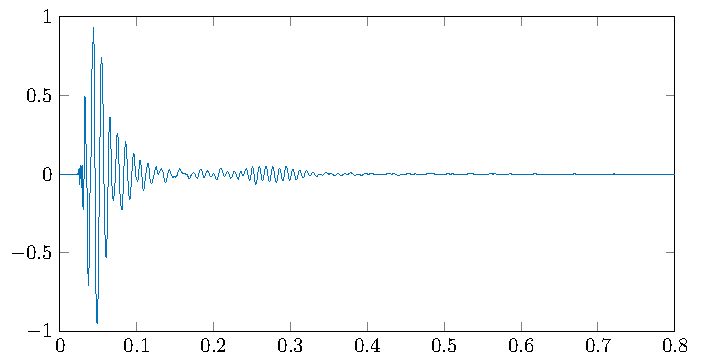
\includegraphics[width=0.9\textwidth]{img/cin/book_time_.pdf}
		\caption{Book fall signal in the time domain.}\label{fig:time_bf}
	\end{subfigure}%
	\begin{subfigure}[ht]{0.5\columnwidth}
		\centering
		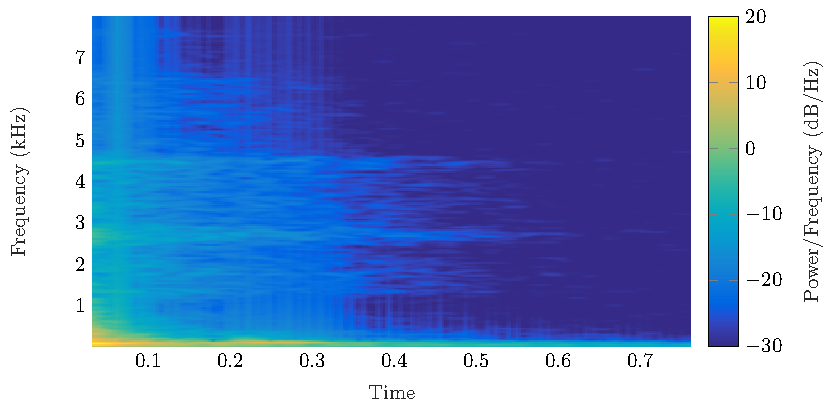
\includegraphics[width=\textwidth]{img/cin/book_freq_.pdf}
		\caption{Book fall signal in the frequency domain.}\label{fig:spec_bf}
	\end{subfigure}
	\caption{Time domain (on the left) and frequency domain (on the right) representation of a normal human activity signal (a-b), human fall signal (c-d), and book fall signal (e-f).}\label{fig:waveforms}
\end{figure}

The algorithm proposed in this work reduces the problem by employing a multi-stage classification approach that combines a one-class classifier based on OCSVM with a template-matching stage. The OCSVM is trained unsupervisedly on a large corpus containing sounds that represent the ``normality''. On the contrary, the template-matching stage employs a set of templates represented by a small number of feature vectors marked as false alarm by the user. Thus, robustness against possible false alarms is achieved by using only few examples of false positive classes without the need of multiple sensors. An additional advantage with respect to the state of the art is that the proposed approach is able to evolve and improve after its initial training, since the template set can be augmented as non-falls events are detected.

\subsection{Proposed approach}
The proposed approach is composed of three stages \figref{fig:overall_ocsvm_user_aided}: the first (``Feature Extraction'') extracts MFCCs from the input audio signal and then GMSs to describe the entire audio segment. The second stage (``Abnormal Event Detection'') consists of a One-Class SVM classifier that discriminates between normal and abnormal sounds. Up to the authors' knowledge, OCSVM together with GMSs have never been jointly used for acoustic fall detection.  The third stage represents the innovative contribution of this work for reducing false alarms in unsupervised approaches: it consists of a ``Template-Matching'' block that refines the output of the OCSVM and classifies the input data as fall or non-fall. The OCSVM is trained unsupervisedly on a large dataset of everyday sounds with the objective of discriminating normal from abnormal sounds. As aforementioned, the basic assumption is that the acoustic events related to human falls are ``rare'' respect to sounds normally occurring inside a home. The template-matching stage, on the other side, requires a set of ``template'' instances that represent rare events that can be confused with a fall. Referring to \figref{fig:overall_ocsvm_user_aided}, the ``Template-Matching'' stage is composed of a set of ``Templates'', a block that calculates the distance between the input GMS and the templates (``Euclidean Distance Calculation''), and a ``Decision'' block the decides whether the event is a fall or a non-fall by evaluating the magnitude of the distance.  The rationale here is that certain acoustic events are as abnormal as falls and confuse the OCSVM: the template-matching stage reduces false positives by using a set of examples related to the most confusing classes. In this work, the algorithm is ``user-aided'', i.e., templates are indicated by the user each time the OCSVM produces a false positive. This is shown in \figref{fig:overall_ocsvm_user_aided} with the person silhouette near the block that decides whether a detected fall is a false positive or not (``False Positive?''). In general, however, it is possible to create the templates set a-priori by recording several instances of possible false alarms events. Although rare, false alarm events (e.g., falls of objects) are certainly easier to reproduce in laboratory respect to human falls.

\subsubsection{Template Matching}
The template-matching classifier operates on a set of templates, i.e., supervectors, that can be defined a-priori or selected by the user when the OCSVM detects an abnormal sound that is not a human fall. Denoting with $\mathbf{x}$ the supervector of the input signal and with $\mathcal{Y} = \{\mathbf{y}_1,\ldots,\mathbf{y}_N\}$ the set of templates, the algorithm operates by calculating the Euclidean distance $D^{(i)} = \| \mathbf{x} - \mathbf{y}_i \|$ between the supervector to be classified and all the templates in the set. Indicating with $D_{min} = \underset{i}{\min}\,\,D^{(i)}$, the supervector $\mathbf{x}$ is classified as a fall if $D_{min}>\beta$ and as non-fall otherwise. The threshold $\beta$ is a hyperparameter of the algorithm that can be determined on a validation set.

\begin{figure}[ht]
	\centering
	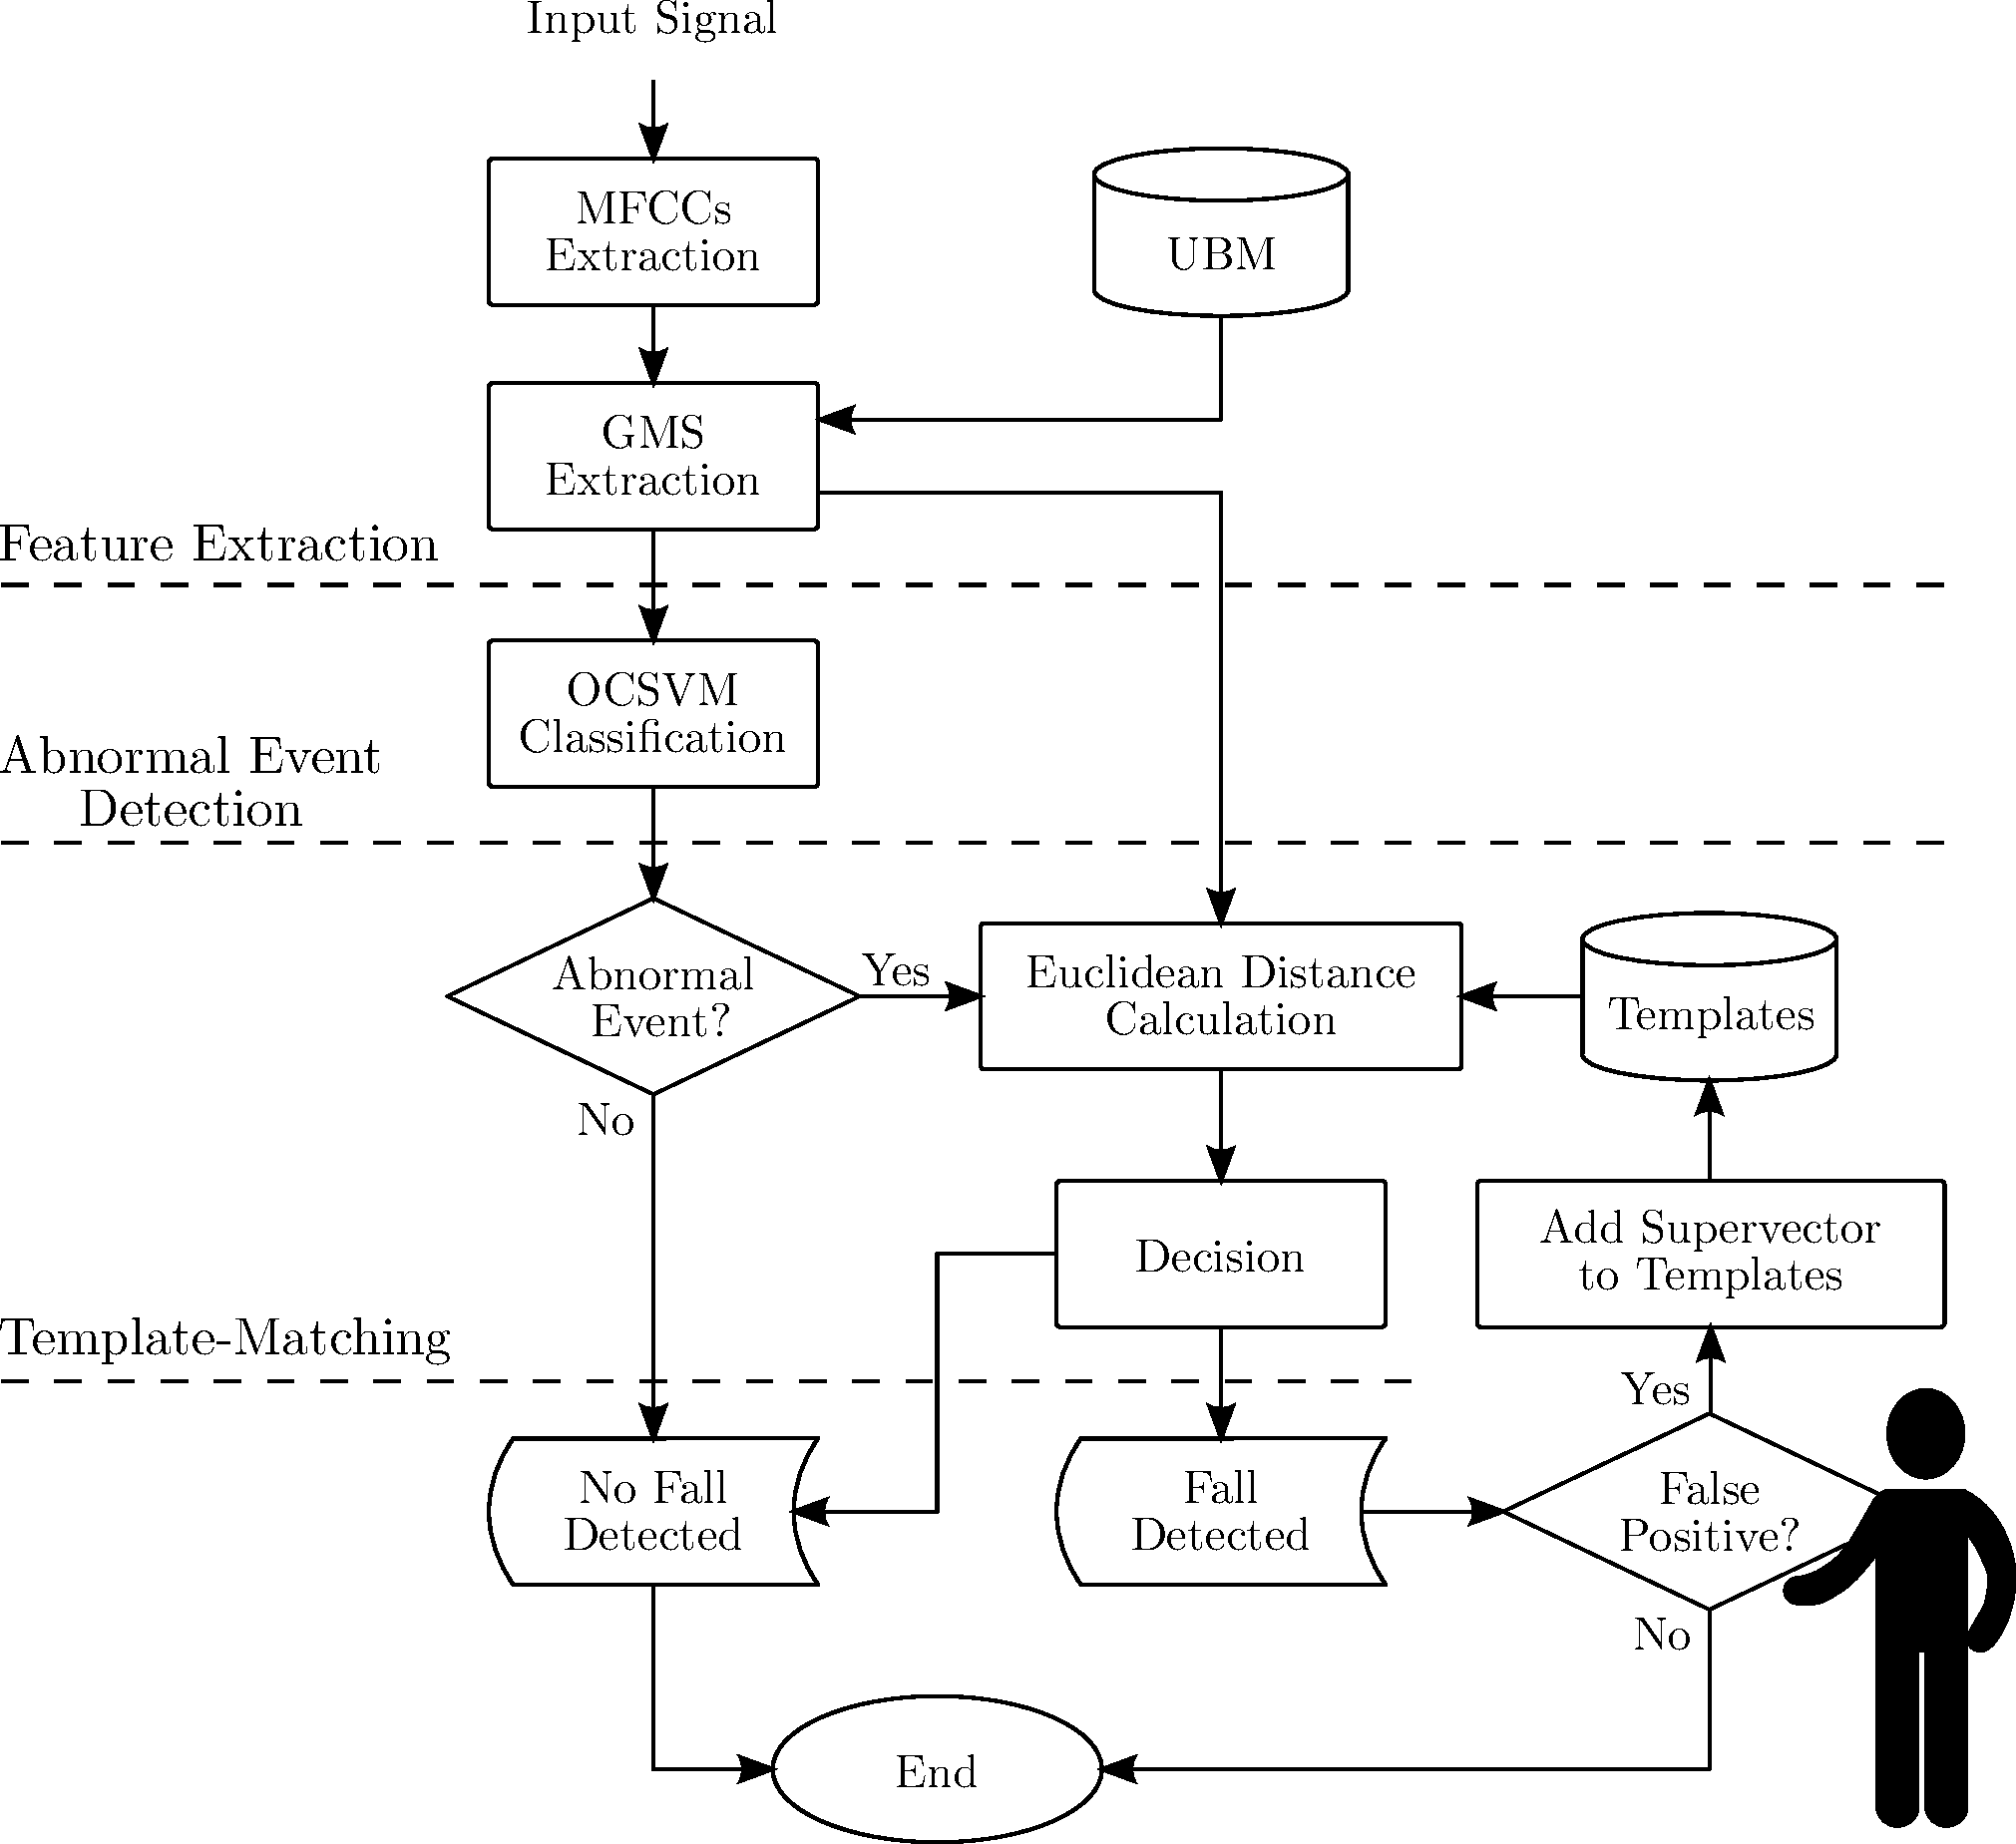
\includegraphics[width=0.95\columnwidth]{img/cin/approccioComplessivo.pdf}
	\caption{The block scheme of the proposed approach.}\label{fig:overall_ocsvm_user_aided}
\end{figure}

\subsection{Dataset}

The dataset employed in this method is the same used for the approach proposed in \secref{sec:ocsvm_approach} and reported in \tableref{tab:ocsvm_dataset}. Please refer to \secref{sec:dataset_cin_ocsvm_only} for the details.

\subsection{Experimental setup}
As in the system presented in \secref{sec:ocsvm_approach}, the dataset has been divided in one set for training the UBM and the OCSVM and three sets for evaluating the performance.
Training has been performed on the same set used for the OCSVM base algorithm presented in \secref{sec:ocsvm_approach} and shown in \tableref{tab:trainComposition}. The same three sets described in \secref{sec:experiment_ocsvm} has been used for the assessment and summarized below as a reminder:
\begin{itemize}
	\item Set 1: Human fall and background sounds (\tableref{tab:set1Composition_}).
	\item Set 2: Human fall and object fall sounds (\tableref{tab:set2Composition_}).
	\item Set 3: Human fall, object fall and background sounds (\tableref{tab:set3Composition_}).
\end{itemize}


\begin{table}[ht]
	\centering
	\caption{Data used in ``Set 1''.}
	\begin{subtable}[ht]{.6\textwidth}
		\centering		
		\caption{Composition  of ``Set 1''.}
		\label{tab:set1Composition_} % è lo stesso del capitolo 5. Lo riporto qui per comodità di lettura
		\begin{center}
			\begin{tabular}{K{3cm}K{3cm}}				
				\hline
				\textbf{Class} & \textbf{Nr.\ of occurrences} \\ 
				\hline
				$\,$ Human Falls $\,$ 	& 44    			\\
				Human Activity  		& 15		\\
				Music			  		& 29		\\
				%				 Classic Music       	& 15   		\\
				%				 Rock Music       		& 14  		\\		
				\hline
			\end{tabular}			
		\end{center}		
	\end{subtable}%
	\begin{subtable}[ht]{.6\textwidth}
		\centering		
		\caption{Templates of ``Set 1''.}\label{tab:set1Template}
		\begin{center}
			\begin{tabular}{ccc}
				
				\hline
				\multirow{2}{1cm}{\textbf{Class}}	& \multicolumn{2}{c}{\textbf{Nr.\ of templates}}	\\ 
				\cline{2-3}
				&\textbf{Clean}&\textbf{Noisy}						\\
				%& \hspace{8pt}Clean\hspace{8pt}  & \hspace{6pt}Clean\hspace{6pt}   \\ 
				\hline
				Human Activity  		& 13	&	11 		\\
				Music       	& 8   	&	16		\\
				%				 Classic Music       	& 8   	&	16		\\
				%				 Rock Music       		& 0  	&	0		\\	
				\hline
				Total					& 21  	&	27		\\
				\hline
			\end{tabular}
			
		\end{center}
	\end{subtable}
	
	
\end{table}

\begin{table}[ht]
	\centering
	\caption{Data used in ``Set 2''.}
	\begin{subtable}[ht]{.6\textwidth}
		\centering
		
		\caption{Composition  of ``Set 2''.}
		\label{tab:set2Composition_}
		\begin{center}
			
			\begin{tabular}{K{3cm}K{3cm}}
				
				\hline
				\textbf{Class} & \textbf{Nr. of occurrences} \\ 
				%& \hspace{8pt}Clean\hspace{8pt}  & \hspace{6pt}Clean\hspace{6pt}   \\ 
				\hline
				$\,$ Human Falls $\,$ 	& 44    		\\				
				Basket      			& 7           	 \\
				Fork        			& 7           	 \\
				Ball       			& 8           	 \\
				Book        			& 7          	  \\
				Bag         			& 8          	  \\
				Chair       			& 7    			\\
				
				\hline
			\end{tabular}
			
		\end{center}
		
	\end{subtable}%
	\begin{subtable}[ht]{.6\textwidth}
		\centering
		
		\caption{Templates of ``Set 2''.}
		\label{tab:set2Template}
		\begin{center}
			\begin{tabular}{ccc}
				
				\hline
				\multirow{2}{1cm}{\textbf{Class}}	& \multicolumn{2}{c}{\textbf{Nr.\ of templates}}	\\ 
				\cline{2-3}
				&\textbf{Clean}&\textbf{Noisy}						\\
				%& \hspace{8pt}Clean\hspace{8pt}  & \hspace{6pt}Clean\hspace{6pt}   \\ 
				\hline
				Basket  		& 55	&	57 		\\
				Fork       	& 39   	&	55		\\
				Ball      		& 11  	&	52		\\	
				Book  			& 26	&	57 		\\
				Bag       		& 26   	&	56		\\
				Chair       	& 86  	&	89		\\
				\hline	
				Total			& 243   &	366		\\	
				\hline
			\end{tabular}
			
		\end{center}
		
		
	\end{subtable}
	
	
\end{table}


\begin{table}[ht]
	\centering
	\caption{Data used in ``Set 3''.}
	\begin{subtable}[ht]{.6\textwidth}
		\centering
		
		\caption{Composition  of ``Set 3''.}
		\label{tab:set3Composition_}
		\begin{center}
			
			\begin{tabular}{K{3cm}K{3cm}}
				
				\hline
				\textbf{Class} & \textbf{Nr. of occurrences} \\ 
				%& \hspace{8pt}Clean\hspace{8pt}  & \hspace{6pt}Clean\hspace{6pt}   \\ 
				\hline
				$\,$ Human Falls $\,$ 	& 44    		\\				
				Basket      			& 3            	\\
				Fork        			& 4            	\\
				Ball       			& 4            	\\
				Book        			& 3            	\\
				Bag         			& 4            	\\
				Chair       			& 4    			\\
				Human Activity  		& 8   			\\
				Music			  		& 14   			\\
				%				 Classic Music       	& 7   			\\
				%				 Rock Music       		& 7   			\\
				
				\hline
			\end{tabular}
			
		\end{center}
		
	\end{subtable}%
	\begin{subtable}[ht]{.6\textwidth}
		\centering
		
		\caption{Templates of ``Set 3''.}
		\label{tab:set3Template}
		\begin{center}
			\begin{tabular}{ccc}				
				\hline
				\multirow{2}{1cm}{\textbf{Class}}	& \multicolumn{2}{c}{\textbf{Nr.\ of templates}}	\\ 
				&\textbf{Clean}&\textbf{Noisy}						\\
				%& \hspace{8pt}Clean\hspace{8pt}  & \hspace{6pt}Clean\hspace{6pt}   \\ 
				\hline
				Basket      			& 52     &  57		\\
				Fork        			& 57     &  57 		\\
				Ball       			& 19     &  55  	\\
				Book        			& 53     &  57   	\\
				Bag         			& 50     &  56    	\\
				Chair       			& 89     &	89		\\
				Human Activity  	& 11   	 &	4		\\
				Music 			      	& 4   	 &	11		\\
				%							 Classic Music       	& 4   	 &	11		\\
				%							 Rock Music       		& 0   	 &	0		\\
				\hline	
				Total						& 335   &	386		\\	
				\hline
			\end{tabular}			
		\end{center}		
	\end{subtable}
	
	
\end{table}
The validation phase has been set following the same procedure described in section \secref{sec:experiment_ocsvm}: a cross-validation composed of four fold has been used for estimating the hyperparameter and  the final performance is calculated by using the cumulative true positives, false positives, and false negatives obtained by varying the test folds.
Differently from the previous method, the validation phase consisted not only in searching for the number of components of the UBM and the parameters ($\nu$ and $\gamma$) of the OCSVM, but also the value of the threshold $\beta$ in the template-matching stage. The values assumed by these variables are summarized in \tableref{tab:parameter}.
The method employed for the template-matching decision threshold is explained in \secref{ssec:templateThreshold}.

%\subsection{Comparative method}

\begin{table}[ht]
	\centering
	\caption{Hyperparameters of the algorithm and search space explored in the validation phase. The search space of the template-matching threshold $\beta$ is not reported, since is determined with the procedure described in \secref{ssec:templateThreshold}. }
	\label{tab:parameter}
	\begin{tabular}{c |c | c}
		\hline
		\textbf{Stage} & \textbf{Hyperparameter} & \textbf{Range} \\
		\hline
		UBM & $J$ & $1, 2, 4, \ldots , 64$\\
		\hline
		\multirow{2}{*}{OCSVM} & $\nu$ & $0.1, 02, \ldots, 1.0$ \\
		&$\gamma$ & $2^{-15}, 2^{-13}, \ldots,2^{3} $ \\
		\hline
		Template-matching & $\beta$  & See \secref{ssec:templateThreshold}\\
		\hline
	\end{tabular}
\end{table}

All the aforementioned datasets require a set of templates for the template-matching stage of the algorithm. In the case of object falls, the set of templates has been created by classifying a set of 372 object falls with the OCSVM and selecting the occurrences misclassified as human falls. In the case of background sounds, the set of templates has been created by calculating the Euclidean distance between each occurrence of the development-set and each occurrence of a set of 470 background signals and then selecting the segment whose distance is minimum. Details on the templates sets are shown in \tableref{tab:set1Template}, \tableref{tab:set2Template}, and \tableref{tab:set3Template} respectively for ``Set 1'', ``Set 2'', and ``Set 3''.


The proposed approach has been compared with the method from which it derives (\secref{sec:ocsvm_approach}) and the algorithm presented in \cite{Popescu2009} based on OCSVM (please revert to \paragref{par:popescu_mod} for the details) 

The performance has been evaluated in terms of F$_1$-Measure \eqref{eq:f1} 

\subsection{Choice of the template-matching decision threshold}\label{ssec:templateThreshold}
A key point of the proposed approach is the decision threshold $\beta$ in the template-matching stage. Choosing a too low value would result in a low number of false negatives and a high number of false positives. On the contrary, a too high value would result in a high number of false negatives and a low number of false positives. The choice of $\beta$ has been performed by calculating the minimum Euclidean distance between each fall and non-fall event in the validation set and the set of templates. \figref{fig:distr_clean} and \figref{fig:distr_noisy} show respectively the probability distributions for the three sets in clean and noisy conditions. The decision threshold $\beta$ has been chosen at the intersection point between the distribution of fall and non-fall distances. This choice represents a compromise that balances false positives and false negatives.

Observing clean condition distributions, in ``Set 1'' the two density are considerably overlapped, while in ``Set 2'' the overlap is modest. It is expected that the possible improvement of the template-matching stage will be more consistent for ``Set 2'' respect to ``Set 1''. ``Set 3'' contains human activity and music occurrences as ``Set 1'' and object falls as ``Set 2'': indeed, the probability distributions (\figref{fig:distr_clean_set3}) are more distinct respect to the ones of ``Set 1'', but not so much as the ones of ``Set 2''.

Noisy condition distributions, shown in \figref{fig:distr_noisy}, are in general less distinct compared to clean condition ones. The effect of noisy is to flatten the distances of the fall and non-fall classes, thus resulting in a less discriminative capabilities of the classifier. Thus, it is expected that the performance improvement in noisy conditions will be more modest respect to the one obtained in clean condition.

\begin{figure}[ht]
	\centering
	\begin{subfigure}{0.9\columnwidth}
		\centering
		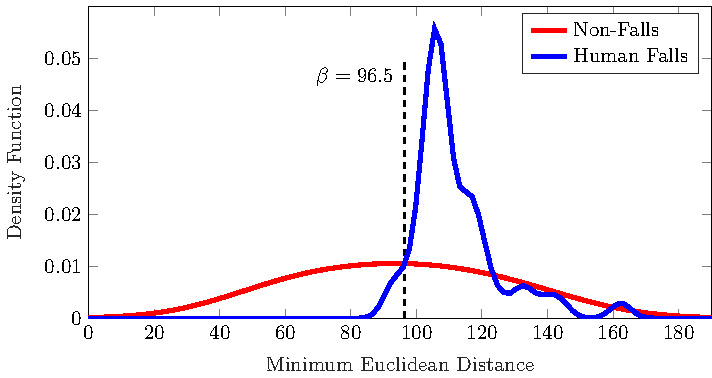
\includegraphics[width=0.98\columnwidth]{img/cin/distribuzione_Caso1_Clean.pdf}
		\subcaption{Probability distributions related to ``Set~1''.}\label{fig:distr_clean_set1}
	\end{subfigure}\hspace{1pt}
	\begin{subfigure}{0.9\columnwidth}
		\centering
		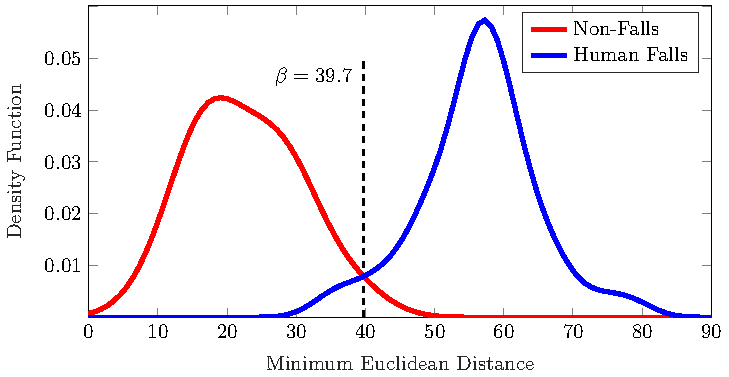
\includegraphics[width=\columnwidth]{img/cin/distribuzione_Caso2_Clean.pdf}
		\subcaption{Probability distributions related to ``Set~2''.}\label{fig:distr_clean_set2}
	\end{subfigure}\hspace{1pt}
	\begin{subfigure}{0.9\columnwidth}
		\centering
		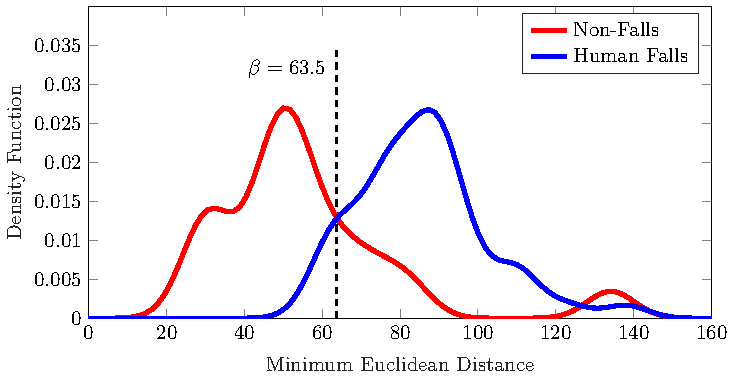
\includegraphics[width=\columnwidth]{img/cin/distribuzione_Caso3_Clean.pdf}
		\subcaption{Probability distributions related to ``Set~3''.}\label{fig:distr_clean_set3}
	\end{subfigure}
	\caption{Probability distributions of the minimum Euclidean distances among the template sets, and human falls and non-falls in \textit{clean} acoustic condition.}\label{fig:distr_clean}
\end{figure}

\begin{figure}[ht]
	\centering
	\begin{subfigure}{0.9\columnwidth}
		\centering
		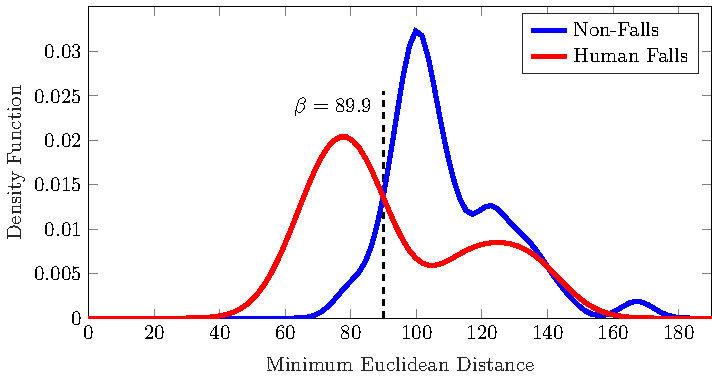
\includegraphics[width=0.98\columnwidth]{img/cin/distribuzione_Caso1_Noisy.pdf}
		\subcaption{Probability distributions related to ``Set~1''.}
	\end{subfigure}\hspace{1pt}
	\begin{subfigure}{0.9\columnwidth}
		\centering
		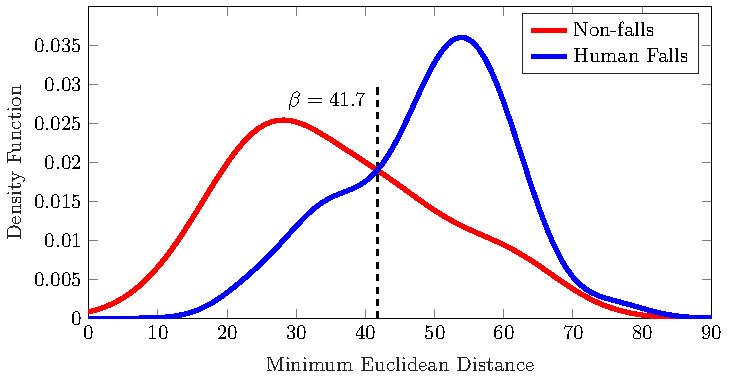
\includegraphics[width=\columnwidth]{img/cin/distribuzione_Caso2_Noisy.pdf}
		\subcaption{Probability distributions related to ``Set~2''.}
	\end{subfigure}\hspace{1pt}
	\begin{subfigure}{0.9\columnwidth}
		\centering
		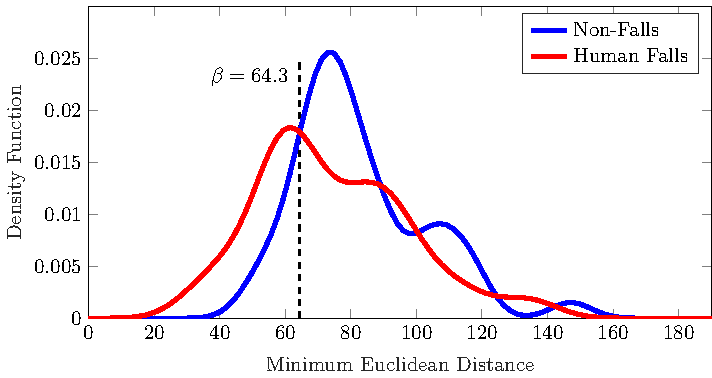
\includegraphics[width=\columnwidth]{img/cin/distribuzione_Caso3_Noisy.pdf}
		\subcaption{Probability distributions related to ``Set~3''.}
	\end{subfigure}%
	\caption{Probability distributions of the minimum Euclidean distances among the template sets, and human falls and non-falls in \textit{noisy} acoustic condition.}\label{fig:distr_noisy}
\end{figure}

\subsection{Results}
\figref{fig:res_clean_} shows the results in clean conditions obtained with and without the template-matching stage, respectively denoted as ``OCSVM+Template-Matching'' and ``OCSVM''. The results obtained with the method proposed in \cite{Popescu2009} are denoted with ``Popescu (2009)''. Observing the figure, it is evident that in all the three cases the template-matching approach is able to improve the performance with respect to ``Popescu (2009)'' \cite{Popescu2009} and the OCSVM only approach. In particular, in ``Set 1'', that comprises human falls, human activities and music, the performance improves by 2.03\% with respect to OCSVM and by 19.64\% with respect to ``Popescu (2009)''. This case can be considered as the least challenging of the three, since non-falls events are considerably different from falls ones. Conversely, ``Set 2'' comprises both human falls and object falls, thus it includes abnormal events whose pattern is similar to the one of human falls. The introduction of the template-matching stage considerably reduces the number of false positives, leading to an overall performance improvement of 20.76\%. ``Set 3'' comprises human falls, human activities, music and object falls and represents the most realistic test condition of the three. Introducing the template-matching stage, the performance improves by 7.64\%, leading to an F$_1$-Measure equal to 89.89\%. 

\begin{figure}[ht]
	\centering
	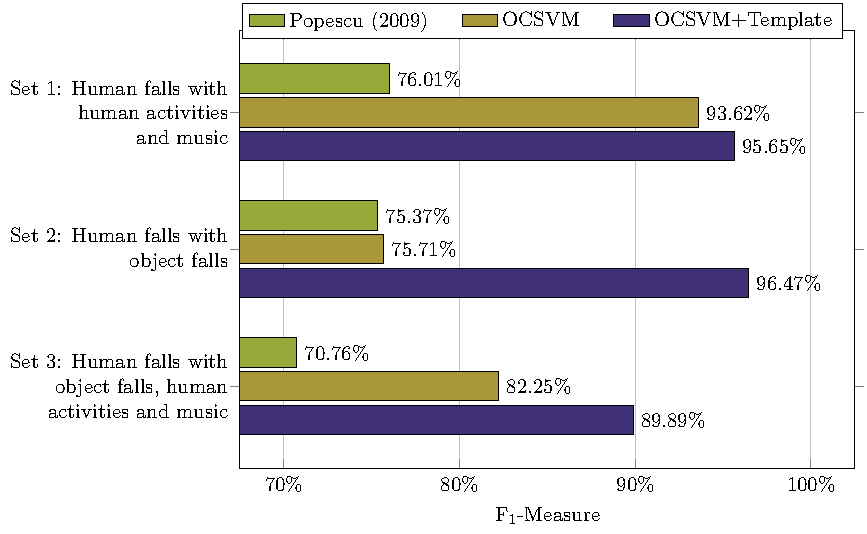
\includegraphics[width=\columnwidth]{img/cin/res_clean.pdf}
	\caption{Results in \textit{clean} conditions for the three test cases. ``Set 1'' comprises human falls, human activities and music. ``Set 2'' comprises human falls and object falls. ``Set 3'' comprises human falls, object falls, human activities, and music.} \label{fig:res_clean_}
\end{figure}

\figref{fig:res_noisy_} shows the results obtained for the three cases in noisy conditions. As expected, the performance decreases in all the three evaluated methods. In ``Set 1'', the performance decrease is modest (2.32\% for the OCSVM, 2.63\% for the proposed approach, and 1.44\% for ``Popescu (2009)''), demonstrating that the OCSVM is able to effectively reject non-fall events corrupted by music interference. The use of the template-matching stage increases the performance by 1.72\%, thus providing a significant improvement also in noisy conditions. In ``Set 2'', Template-matching provides a performance improvement of 8.02\% with respect to the OCSVM, leading to an F$_1$-Measure higher than 70\%. The improvement is lower with respect to the clean ``Set 2'', since the variability of the music interference makes the Euclidean distances of fall and non-fall classes more similar and is not sufficient to overcome the ``Popescu (2009)'' \cite{Popescu2009}. In ``Set 3'', the proposed approach improves the performance by 4.77\% with respect to OCSVM and by 8.68\% with respect to ``Popescu (2009)''.

In summary, the results demonstrated that the introduction of a template-matching stage significantly improves the performance both of the OCSVM only approach and of the method by Popescu and Mahnot \cite{Popescu2009}: averaging the results over ``Set 1'', ``Set 2'', and ``Set 3'', the absolute improvement with respect to the former is 10.14\% in clean conditions and 4.84\% in noisy conditions. With respect to the latter \cite{Popescu2009} the improvement is 19.96\% in clean conditions and 8.08\% in noisy conditions. As shown in \figref{fig:res_clean_} and \figref{fig:res_noisy_}, both in clean and noisy conditions the F$_1$-Measure of the method by Popescu and Mahnot \cite{Popescu2009} is close to 75\% in ``Set 1'' and ``Set 2'', and close to 71\% in ``Set 3''. The different behaviour compared to the OCSVM only approach can be attributed firstly to the different feature representation of the audio signal (MFCCs instead of supervectors). Secondly, to the strategy adopted for classification: in \cite{Popescu2009}, signals are divided in windows and a fall is detected if at least two consecutive windows are classified as fall. Differently, in the proposed algorithm, the overall signal is represented by a single supervector and classified as fall or non fall.

Comparing the results in clean (\figref{fig:res_clean_}) and noisy (\figref{fig:res_noisy_}) conditions, it is evident that techniques for reducing the impact of additive noise are needed. Additionally, the proposed solution requires the intervention of the user for selecting the templates after the first classification stage performed by the OCSVM. This aspect will be addressed in next sections in order to make the algorithm completely independent of the user, using a low number of examples related to human fall.

\begin{figure}[ht]
	\centering
	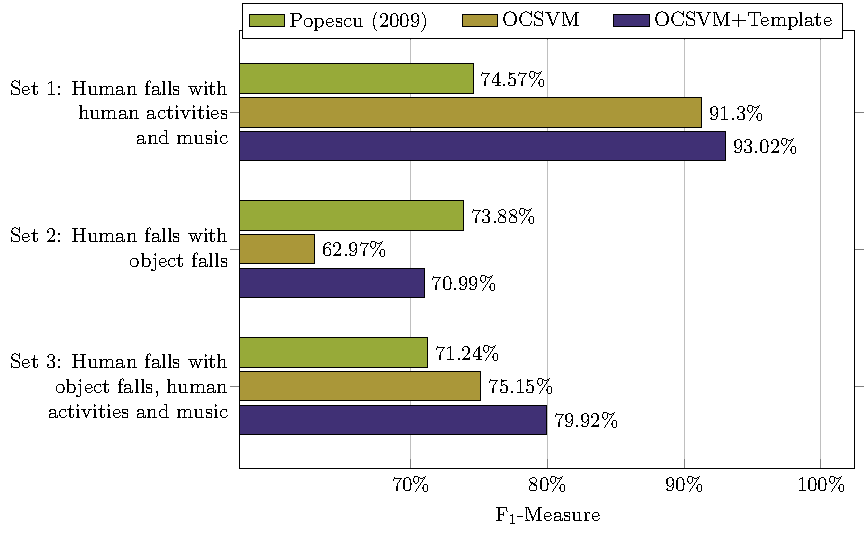
\includegraphics[width=\columnwidth]{img/cin/res_noisy.pdf}
	\caption{Results in noisy conditions for the three test cases. ``Set 1'' comprises human falls, human activities and music. ``Set 2'' comprises human falls and object falls. ``Set 3'' comprises human falls, object falls, human activities, and music.} \label{fig:res_noisy_}
\end{figure}


\section{Few-shot Siamese Neural Networks employing Audio features for Human-Fall Detection}
\label{sec:siamese_few_shot}
As already mentioned, the main challenge for falls detector systems is the lack of human falls examples in the dataset, that are rare and hardly recoverable. Hence the need to develop systems that are able to work with no or few such data. In fact, Khan et al. \cite{khan2017review} analyze Fall Detection techniques and divides them based on data availability prospective in two groups. The group is composed of algorithms that can draw form dataset with sufficient number of human falls that can be used in training. Mostly based on supervised machine learning, thresholding and one-class techniques, this methods attempt to detect a fall directly given their training data. As we show here, although these supervised techniques can achieve a high reliability, they needs a large labelled dataset including many human fall, that is not easy to retrieve for this specific application. Moreover, applying this techniques when there are no training data for human falls leads to an unacceptable miss rate. As a comparative model for this category, has been evaluated an algorithm based on SVM.% described below %that shows good results in \cite{Principi2016a}
. The second group include algorithms that can draw form dataset with insufficient or no training data for falls mostly based on over/under-sampling, semi-supervised learning, novelty detection and one-class classification. Those techniques differ from the previous ones because uses the available data as a description of normal activities. Once it is trained on these data, can be able to classify a test sample as a human fall or non-human fall. The major drawback here is that they need a good description of what ``normal activities'' are. In fact to give a good representation of this concept, a big data set comprising all the normal activities is needed \cite{pimentel2014review}. In real scenario, this is very difficult to obtain and this may induce the classifier to produce a high number of false alarms. As a comparative models for this category, 2 approaches have been evaluated: a OCSVM that is a totally unsupervised method and a extremely unbalanced SVM that use only one human fall for the training phase%, both described below.
.

The proposed algorithm belongs to the second category, and as a first step, we demonstrate that the SNN can achieve better results than both unsupervised and supervised methods when they are tested under similar conditions.


%Learning a Similarity Metric Discriminatively, with Application to Face Verification
% quello di lecunn e ella contrastive loss
%One-Shot Learning of Object Categories 
% del 2006
%One-shot Learning with Memory-Augmented Neural Networks
%altro lavoro su one shot learning
%Matching Networks for One Shot Learning
%altri lavori sepre su immagini per il one shot (non siamesi)
One-shot or few-shot methods have been recently revived in other fields of application.
The Siamese approach was introduced by Bromley et al. \cite{bromley1994signature} for signature verification and later also used in \cite{chopra2005learning} for face verification, both of them in a supervised framework. Regarding the one-shot learning approach, the Siamese framework was first employed by Koch et al.\cite{koch2015siamese} for image recognition.
In \cite{vinyals2016matching} an attention mechanism over a learned metrics is used. In that work, the authors propose so-called Matching Networks trained by showing only a few examples per class for each minibatch in order to mimic the few-shot task by subsampling classes in a meta-learning perspective.
In the audio field, one-shot approaches have been rarely used up to now.
Lake et al. \cite{lake2014one} proposed a hierarchical Bayesian acoustic-based approach to model the way a person learns a word of a new language from a few examples. They use a Hierarchical Hidden Markov model that induces the set of phone-like acoustic units directly from the raw unsegmented speech data in a completely unsupervised manner, identifying segments that should be clustered together and learning a set of phone-like acoustic units for the language.
Manocha et al.\cite{manocha2017content} proposed a method based on Siamese networks for audio Content-based Representations.

\section{Proposed Approach}
\label{sec:proposed_app}
%In this work the authors applied a Siamese Neural Network 
In this work the authors propose a Siamese Neural Network able to learn a latent representation of an audio event. In particular, a SNN is composed of two twin networks with binded weights. A pair of inputs is provided to the system, one to each twin network. Downstream, the network maps these inputs into two different representation vectors. Then, a certain type of distance between those two representations is computed. In this work euclidean distance was used. In \figref{proposed_approach}, are reported two example of mel-spectrograms: the spectrum that is given as input to the function first network represents a chair that is overturned. The other inputs instead represent a human fall. As can be seen, the signals are not distinguishable at a glance, thus we think that the differential approach of the SNN, described below, seems to be appropriate.

Consider $X_1$, $X_2$ as a pair of two input samples and $Y(X_1, X_2)$ as the label assigned to this pair, we assign $Y = 0$ (positive example) if the inputs $X_1$ and $X_2$ are from the same distribution, $Y = 1$ (negative example) otherwise. The euclidean distance between the mapping $S_e(X_1)$ and $S_e(X_2)$ performed by the network is defined as:
\begin{equation}
E_w = \norm{S_e (X_1) - S_e (X_2)}.
\end{equation}\\
The training procedure consists in minimize the differences of $X_1$, $X_2$ for inputs belonging to the same class ($Y = 0$) while maximize the differences for inputs of different classes ($Y = 1$). % In fact, entire network is trained in such a way to learn inputs differences, predicting 1 if the two input are not from the same distributions and 0 (negative example) if the input are from the same distributions (positive example).
The loss function used to achieve this minimization is the contrastive loss, described by LeCun et al. in \cite{chopra2005learning}:
\begin{equation}
Loss = (1 - Y)\frac{1}{2}(E_w)^2 + (Y)\frac{1}{2}\{(max(0, m - E_w)\}^2 .
\end{equation}\\
Here the parameter $m > 0$ is the \textit{margin} that allows only negative examples whose distance is less than the radius defined by $m$ itself, to contribute to the loss function.
In this way the system should be able to learn embedded features allowing classification even of the unseen rare sound event such as human fall.
%Dire che questo tipo di approccio, dovendo combinare in ingesso gli esempi a disposizione, permette un aumento del trainset, vantaggioso nel caso in cui si opera con dataset piccoli.
Our Siamese network has been trained on a corpus of labelled object fall events and not including any human fall. Pairs of events belonging to the same class correspond to the positive examples while pairs of events belonging to the different class a negative one as explained in section \ref{sec:dataselection}. In particular, the term few-shot comes from the fact that although, in this case study, human falls have not been used for training, some of them are used in the optimization phase, before the final test.
\begin{figure*}
	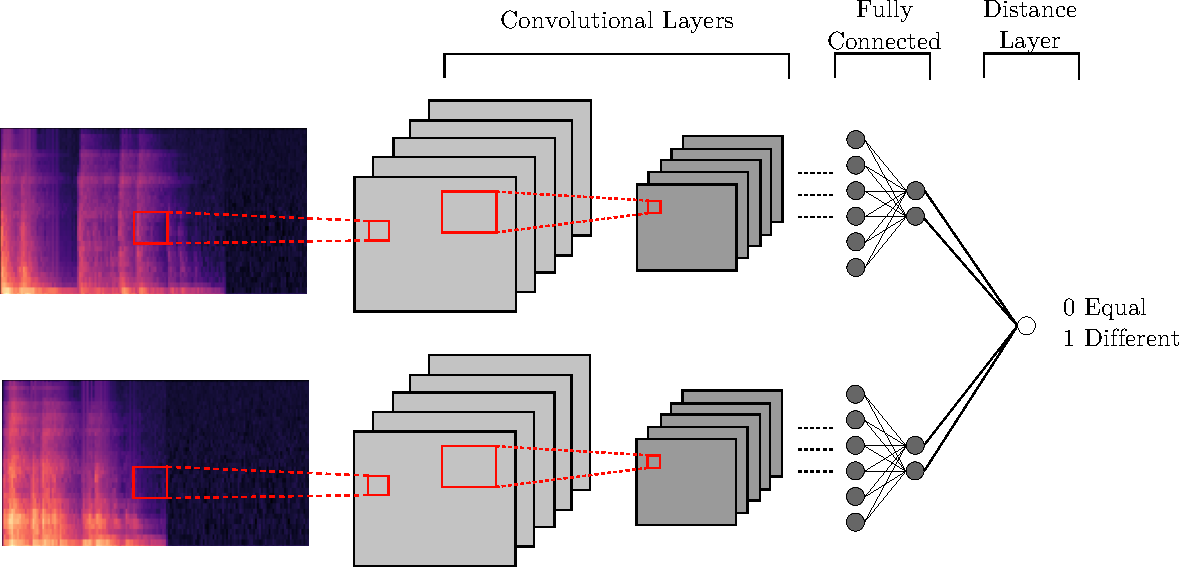
\includegraphics[width=\linewidth]{img/prai/Siamese_approach}
	\caption{Proposed approach.}
	\label{proposed_approach}
	% i mel spect sono rndy_d4st_chair_2.wav e chair_d6h0_side_5.wav
	
\end{figure*}
\subsection{Feature Extraction}
The example provided to the system are preprocessed in a features extraction stage that computes the log mel-energies. These features have been chosen as they are very popular for computational audio analysis \cite{gemmeke2013exemplar,parascandolo2017convolutional,mesaros2010acoustic}.
In particular, for this work the log mel-energies have been computed as follows.
First the signals were padded with some AWGN samples to the length of the longest audio event present in the dataset in order to work with the designed neural network.
Then the audio has been downsampled to 16 kHz and normalized. After that signal has been segmented in frames 40 ms long overlapped
by 20 ms and multiplied with a Hamming window. Discrete Fourier Transform (DFT) is calculated and the absolute value is filtered with a filterbank composed of 40 triangular filters uniformly spaced on the mel scale. At the end each audio event is represented as a matrix $X$ of shape $40\times159$.  

\subsection{Network Architecture}
As shown in \figref{proposed_approach}, the architecture explored here for the twin networks consists of $L_c$ convolutional layers followed by a max pooling. After the convolutional part, there are $L_f$ fully connected layers. After each convolutional and fully-connected layers a \textsl{batch normalization} on features map is applied followed by a \textsl{Leaky ReLU} activation function.
See \secref{sec:Results} for details about the best performing network. 



\subsection{Dataset}
All the instances related to the fall events of the R0 room (\secref{sec:dataset}) has been used in this work. In order to achieve a data augmentation, the instances recorded with all the microphones used during the creation of the dataset has been used:
\begin{itemize}
	\item one microphone array composed of 3 microphones (here taken as single microphones);
	\item 2 prototype of Floor Acoustic Sensor: the first, from now on indicated with FAS, was widely described and used in previous works \cite{Principi2016a} (\figref{fig:FAS}). For the second the only difference is the microphone used inside\footnote{RODE Lavalier: http://en.rode.com/microphones/lavalier.} that is characterized by an omni-directional directivity pattern instead of hyper-cardioid pattern.
\end{itemize}

\tableref{tab:numDataset_few_shot} shows the number of instances for each class used in this work considering only audio recorded with FAS. 
%\begin{figure}
%	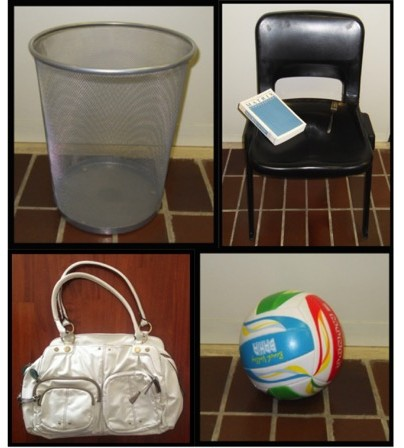
\includegraphics[width=\linewidth]{images/oggetti_cadute3.jpeg}
%	\caption{Objects used during the data acquisition camping.}
%	\label{fig:objects}
%\end{figure}
%\begin{figure}
%	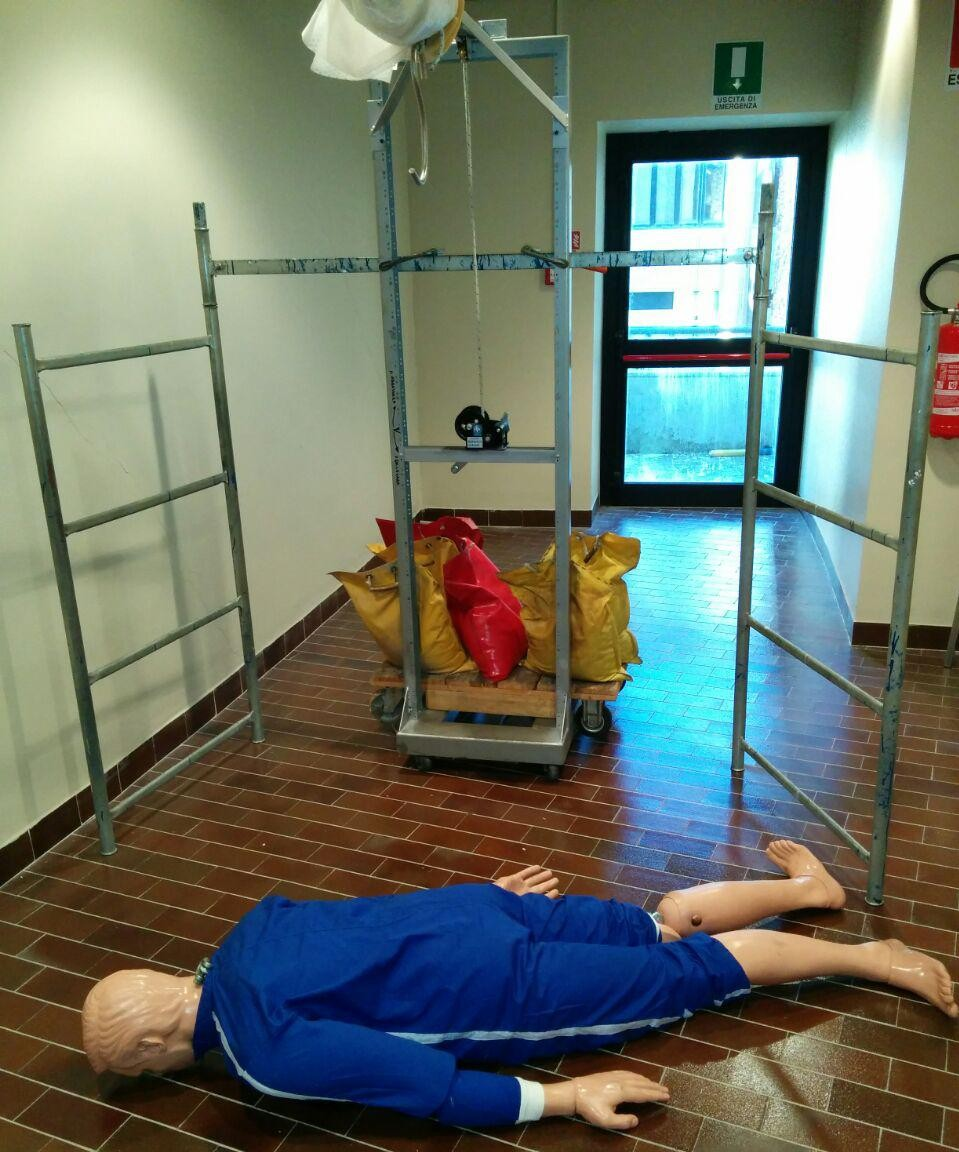
\includegraphics[width=\linewidth]{images/impalcatura.jpg}
%	\caption{Mimikin doll used to simulate the human falls.}
%	\label{fig:mimikin_doll}
%\end{figure}

\begin{table}[ht]
	\caption{Composition  of the dataset.}
	\label{tab:numDataset_few_shot}
	\begin{center}
		%		\begin{tabular}[ht]{c>{\centering}m{5cm}c}
		\begin{tabular}[ht]{c|c|c}	
			\hline
			\textbf{Class} & \textbf{Nr. of occurrences} & \textbf{Total length (s)} \\ %\cline{2-5} 
			%& \hspace{8pt}Clean\hspace{8pt}  & \hspace{6pt}Clean\hspace{6pt}   \\ 
			\hline
			Basket      			& 64    &   86    	\\
			Fork        			& 64    &   82     	\\
			Ball       				& 64    &   129     \\
			Book        			& 64    &   63    	\\
			Bag         			& 64    &   57     	\\
			Chair       			& 96    &   157     \\
			$\,$ Human Falls $\,$ 	& 44    &   76     	\\
			%Human Activity  		& 665   &   1218     \\
			%Music					& 776   &	1498	\\
			%				 Classic Music       	& 441   &   882     \\
			%				 Rock Music       		& 335   &   616     \\
			\hline
		\end{tabular}
	\end{center}
\end{table}


\section{Experiments}
\label{sec:experiments}


Two methods previously described have been taken as a baseline for the comparison:
in \secref{sec:biclass_svm} a supervised approach based on bi-class SVM able to discriminate fall event from  non-fall event was employed. In this works the training set was composed of labeled data representing fall and non-fall event. In \secref{sec:ocsvm_approach} instead, an unsupervised method based on OCSVM was presented. In this case the training set was composed only from background that comprises human daily activities sounds, classical and rock music played from a loudspeaker.
.
For a correct comparison baseline, experiments have been repeated using the same data employed here for the SNN %but with some difference dependent on the type of the algorithm 
as described below \secref{sec:dataselection}.

\subsubsection{Data Selection}
\label{sec:dataselection}
All the experiments have been conducted with three-way data split and a 10 folds cross-validation strategy. In particular, for each fold, the data has been divided in 90\% for indicated, 5\% for validation and 5\% for the test, so in each set, all the classes indicated in the \tableref{tab:numDataset_few_shot}, are present in a balanced way. Since here we approach the problem as a binary classification, this has led, of course, to an imbalance between the human fall and the rest% detto perchè poi mi serve per giustiicare i fatto dela confusion matrix cumulativa 
.
Because each evaluated approach differs from the other, it was necessary to select the data for each of them. To keep the various experiments comparable to each other, starting from the set above, we have constructed the various data sets for each approach as follows:
\begin{itemize}
	\item SNN: first all the signals corresponding to the human fall class have been removed from the training set. Inasmuch as the Siamese network works with paired inputs we generated all the combinations, without repetitions, between all the training examples and then randomly 80000 pairs were selected. In prediction phase, the Siamese Network needs a template to classify the events, so the development set has been subdivided in sub-test: in each of these a human fall present in the validation set has been paired with all the other events present in the same set. In the test, instead, a single human fall was selected randomly to be used as a template for each fold. This was done to keep the test set comparable between the different methods;
	\item SVM: no changes have been made to the lists;
	\item SVM-unbalanced: in the training set only a human fall has been left;
	\item OCSVM: as this is an unsupervised method all the signals corresponding to the human fall class have been removed from the training set.
\end{itemize}
For each method, the development and test set have been used only the FAS signals while the training set has been augmented with the instances of the events recorded with all others the microphones. 



\subsubsection{Validation and Evaluation}

The performances of the compared algorithm have been evaluated in term of $ F_1 -Measure$ referred to the human fall class. Due to the unbalanced nature of development and test set, the metric has been computed starting from a normalized confusion matrix. In particular, for the final evaluation, all the absolute confusion matrices coming from each fold have been summed. The cumulative confusion matrix has been then normalized and the final  $ F_1 -Measure$ was computed from it. 

To optimize the hyper-parameters of the methods the following strategies have been adopted:
\begin{itemize}
	\item for the SNN a small random search of 30 network configurations has been performed. The hyper-parameters varied during the search are reported in \tableref{tab:random_search_params}.
	The search of the threshold value of the output layer of the network which yielded the best $ F_1 -Measure$ has been performed on the validation set.
	%	 During the computation of the $ F_1 -Measure$ on the development set, optimum threshold search for the output layer of the network have been performed.
	The threshold found in this way was then used for the test of the same fold;
	\item for the SVM methods a grid search strategy has been adopted to optimize the parameters. In particular the parameters have assumed values in the ranges  $\{ 2^{-5},2^{-3},\ldots,2^{15} \}$ for $ C $ (SVM) and $ \nu $ (OCSVM), $\{ 2^{-15},\\2^{-13},\ldots,2^{3} \}$ for $ \gamma $ (both SVM and OCSVM) and  $\{ 1,2,\\\ldots,64 \}$ for the number of mixture of the GMM-UBM. 
	The parameter's values that led to the highest result were then used during the test of the same fold.
\end{itemize}

For the Siamese network, a Glorot uniform weight initializer has been used for all layers. Adadelta has been used as optimizer algorithm with default initial parameters \cite{zeiler2012adadelta}. Different values of learning rate decay have been tried in the random-search.
We trained the network for a maximum of 300 epochs, but an early stopping on the $ F_1 -Measure$ has been used to interrupt training if there were no improvements for 25 consecutive epochs. At the ends, the model corresponding to the epoch that gave the best result was selected for the evaluation on the test set.

\begin{table}[ht]
	\caption{Hyper-parameters optimized in the random-search phase, and their range.}\label{tab:random_search_params}
	\centering
	
	\begin{tabular} {|K{4cm}|K{4cm}|}
		\hline
		\textbf{Parameter} 		& \textbf{Range} \\  
		\hline
		Cnn layer Nr. 	& [2-5]		                          \\
		\hline
		Kernel shape 	& [3x3-9x9]  \footnotemark[3]      \\
		\hline									
		Kernel Nr. 		& [8-256]	                            \\
		\hline                      
		MLP layers Nr. 	&	[1-5]	                          \\
		\hline
		MLP layers dim.	&[30-8000]                            \\
		\hline
		Stride & [1x1-2x2]			                          \\
		\hline
		Dilation & [1x1-20x20]\footnotemark[3]   \\
		\hline
		Batch size	&	[100-2000]                                    						\\
		\hline 
		Max pool shape & [1x1-5x5]\footnotemark[3]      \\
		\hline
		Dropout & [Yes-No]     \tablefootnote{For all layers.}               \\
		\hline
		Drop rate	&	[0.3-0.8]                         \\
		\hline
		Learning rate decay	&	[$0$-$0.2$] \% \tablefootnote{After each epoch.}    \\
		\hline                
		Batch normalization	&	[Yes-No]                    \\
		\hline
		
	\end{tabular}
\end{table}

\footnotetext[5]{Also not squared shape has been used.}

\footnotetext[6]{Value in the square brackets represents the value adopted for each layer.}

\section{Results}
\label{sec:Results}
The results obtained for each method are reported in \figref{fig:results_f1}. The figure shows the $ F_1 -Measure$, false negative rate (miss rate) and false positive rate (false alarm rate) referred to the human fall class. It is clear that the supervised SVM method outperforms all other in terms of  $ F_1 -Measure$ as expected. The OCSVM instead is the worst method if used in this context, because its training procedure does not include any human fall, but the normality model is composed of others types of falls, making it difficult to identify the human fall as ``novelty''. The Siamese and the SVM-unbalanced, which start from the same data for the training, are classified in the intermediate positions as expected. However, we note that the proposed approach achieves a better result, exceeding the $ F_1 -Measure$ of SVM-unbalanced of about 11\%. 

As the fall detection is a task that needs to give a higher weight to the miss with respect to the false alarm, \figref{fig:results_fn_fp} reports those metrics. 
Here can be seen that both SVMs methods outperform the others, obtaining an optimum false alarm rate of 0\%. For the Miss rate, instead, while SVM reach a good result of 11\%, SVM-unbalanced give an unacceptable result of about 50\%.
The Siamese network behaves in an opposite manner with respect to the SVM-unbalanced. Although it has an high false alarm rate, it manages to reduce to zero the miss rate.
For a complete overview of the scores, in \cref{tab:cm_svm,tab:cm_svmo,tab:cm_ocsvm,tab:cm_ocsvm} are reported the normalized confusion matrix.

Another consideration is about the generalization capacity of these 4 methods. \figref{fig:score_val_test} reports the score achieved by the algorithms for both validation and test set in the 10 folds. 
The trends show that while for the SVM there is always a set of hyper-parameter able to achieve a 100 $ F_1 -Measure$ in validation phase, this does not happen for the SVM-unbalanced due to the lack of human falls during the training phase. Moreover, the results of validation are not always similar to the test value. The OCSVM instead, have a stable performance in validation, but they drop during the test, showing the poor generalization capacity of the algorithm. 
For the proposed method, instead, the trends in test follow closely the validation ones. This is highlighted in \figref{fig:diff_test_validation} where the trends of the differences in the results between the tests and validations score are shown.

	\begin{figure}
	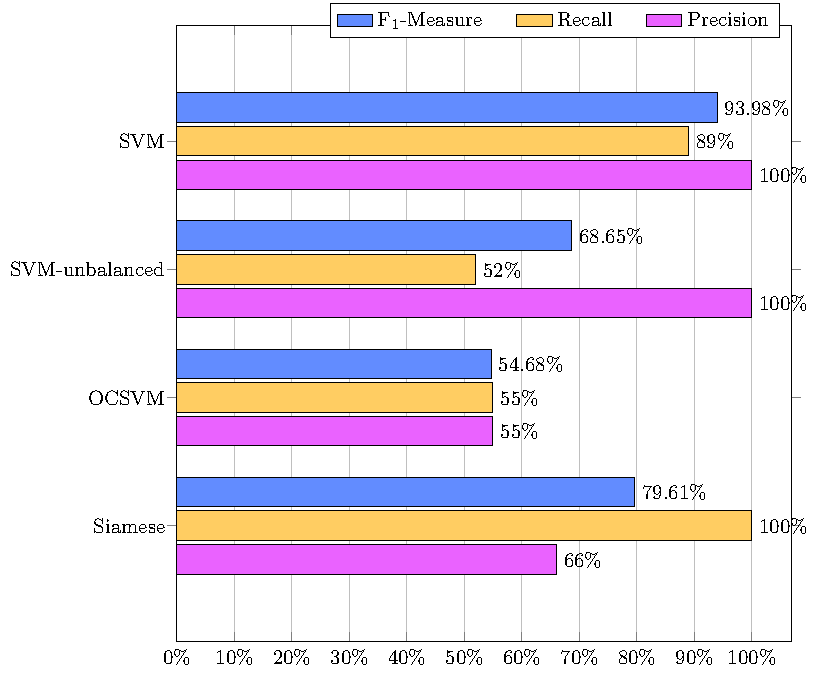
\includegraphics[width=\linewidth]{img/prai/results_f1/results_f1}
	\caption{$ F_1 -Measure$, precision and recall: the metrics are referred to the human fall class}
	\label{fig:results_f1}
\end{figure}
\begin{figure}
	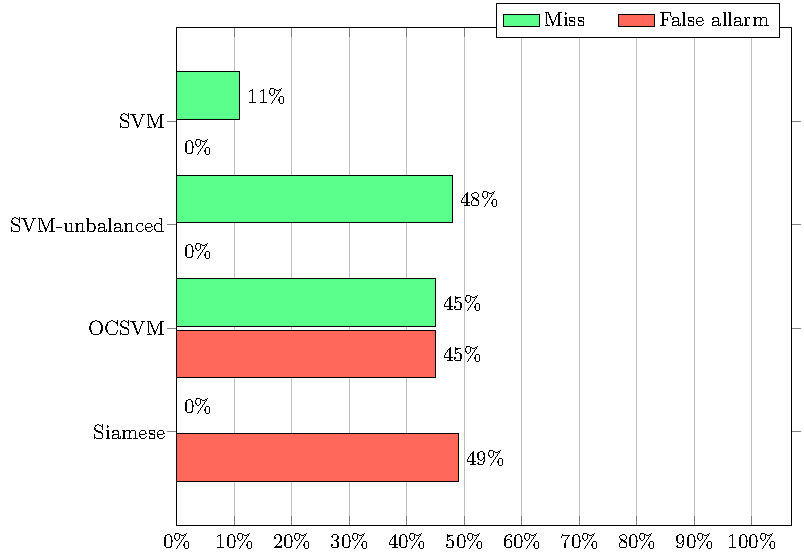
\includegraphics[width=\linewidth]{img/prai/results_fn_fp/results_fn_fp}
	\caption{Miss and false alarm rate: the metrics are referred to the human fall class}
	\label{fig:results_fn_fp}
\end{figure}
\begin{table}[ht]
	\caption{Normalized confusion matrix of the SVM approach.}
	\label{tab:cm_svm}
	\begin{center}
		
		\begin{tabular}[ht]{c|c|c}	
			\hline
			\textbf{\%} & \textbf{$\,$ Human Falls $\,$ } & \textbf{Objects} \\ %\cline{2-5} 
			
			\hline
			\textbf{$\,$ Human Falls $\,$ }     			& 89    &   11     \\
			\textbf{Objects} 								& 0    &   100     	\\
			\hline
		\end{tabular}
	\end{center}
\end{table}
\begin{table}[ht]
	\caption{Normalized confusion matrix of the SVM-unbalanced approach.}
	\label{tab:cm_svmo}
	\begin{center}
		
		\begin{tabular}[ht]{c|c|c}	
			\hline
			\textbf{\%} & \textbf{$\,$ Human Falls $\,$ } & \textbf{Objects} \\ %\cline{2-5} 
			
			\hline
			\textbf{$\,$ Human Falls $\,$ }     			& 52    &   48     \\
			\textbf{Objects} 								& 0    &   100     	\\
			\hline
		\end{tabular}
	\end{center}
\end{table}
\begin{table}[ht]
	\caption{Normalized confusion matrix of the OCSVM approach.}
	\label{tab:cm_ocsvm}
	\begin{center}
		
		\begin{tabular}[ht]{c|c|c}	
			\hline
			\textbf{\%} & \textbf{$\,$ Human Falls $\,$ } & \textbf{Objects} \\ %\cline{2-5} 
			
			\hline
			\textbf{$\,$ Human Falls $\,$ }     			& 55    &   45     \\
			\textbf{Objects} 								& 45    &   55     \\
			\hline
		\end{tabular}
	\end{center}
\end{table}
\begin{table}[ht]
	\caption{Normalized confusion matrix of the Siamese Neural Network approach.}
	\label{tab:cm_siamese}
	\begin{center}
		\begin{tabular}[ht]{c|c|c}	
			\hline
			\textbf{\%} & \textbf{$\,$ Human Falls $\,$ } & \textbf{Objects} \\ %\cline{2-5} 
			\hline
			\textbf{$\,$ Human Falls $\,$ }     			& 100    &   0     \\
			\textbf{Objects} 								& 51     &   49    \\
			\hline
		\end{tabular}
	\end{center}
\end{table}

\begin{figure}[ht]
	\centering
	\begin{subfigure}[b]{0.48\textwidth}
		\centering
		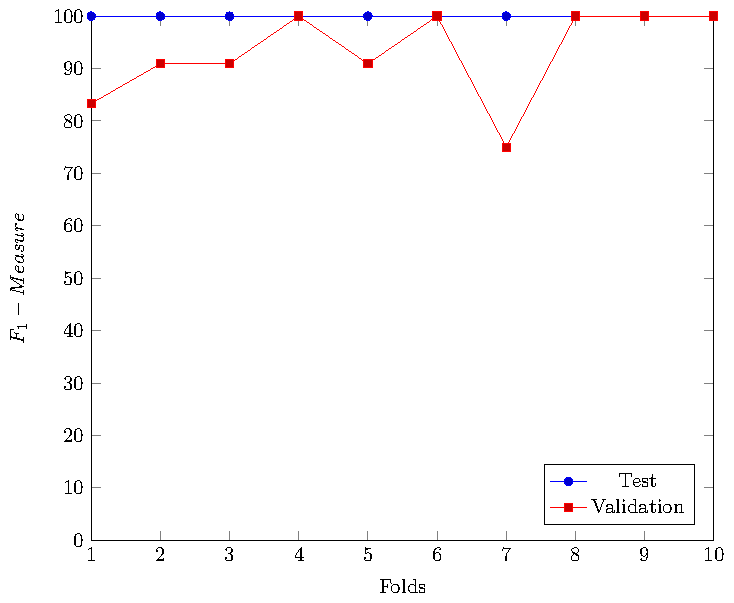
\includegraphics[width=\textwidth]{img/prai/svm_test_validation/svm_test_validation}
		\caption[Network2]%
		{{\small SVM}}    
		\label{fig:svm_val_test}
	\end{subfigure}
	\hfill
	\begin{subfigure}[b]{0.48\textwidth}  
		\centering 
		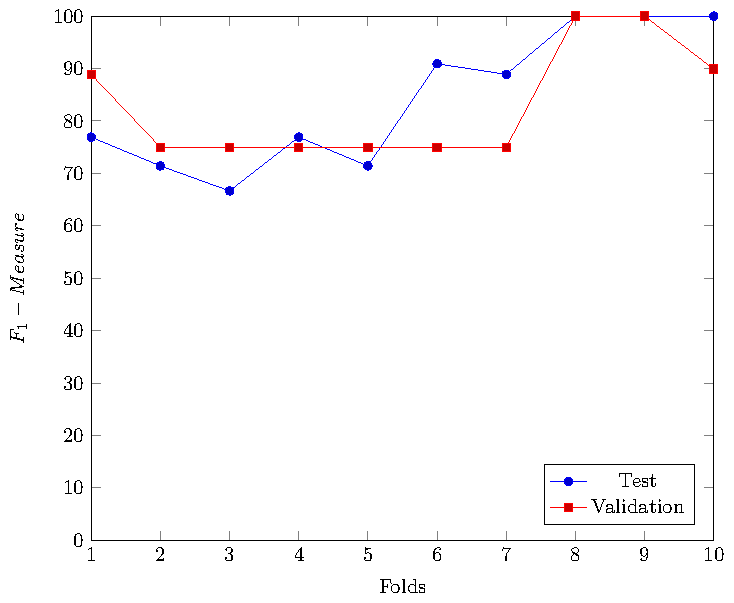
\includegraphics[width=\textwidth]{img/prai/svm_unbalanced_test_validation/svm_unbalanced_test_validation}
		\caption[]%
		{{\small SVM-unbalanced}}    
		\label{fig:svm_unb_val_test}
	\end{subfigure}
	\vskip\baselineskip
	\begin{subfigure}[b]{0.48\textwidth}   
		\centering 
		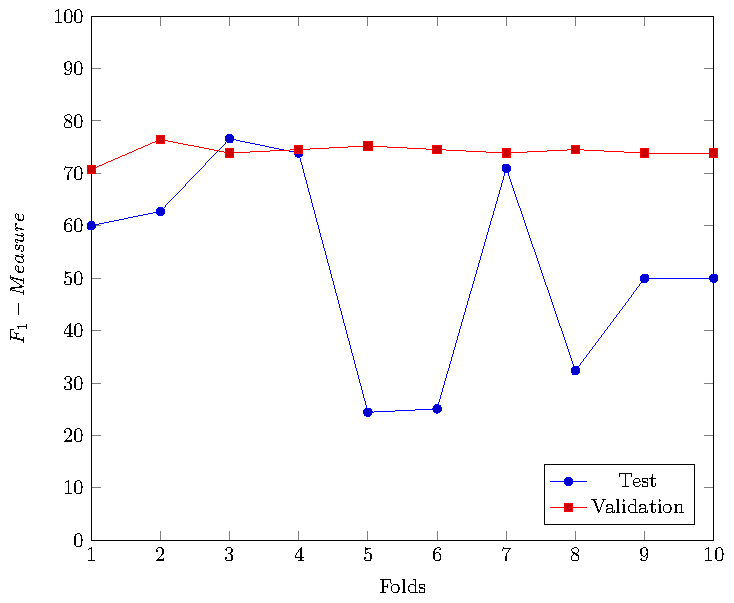
\includegraphics[width=\textwidth]{img/prai/ocsvm_test_validation/ocsvm_test_validation}
		\caption[]%
		{{\small OCSVM}}    
		\label{fig:ocsvm_val_test}
	\end{subfigure}
	\quad
	\begin{subfigure}[b]{0.48\textwidth}   
		\centering 
		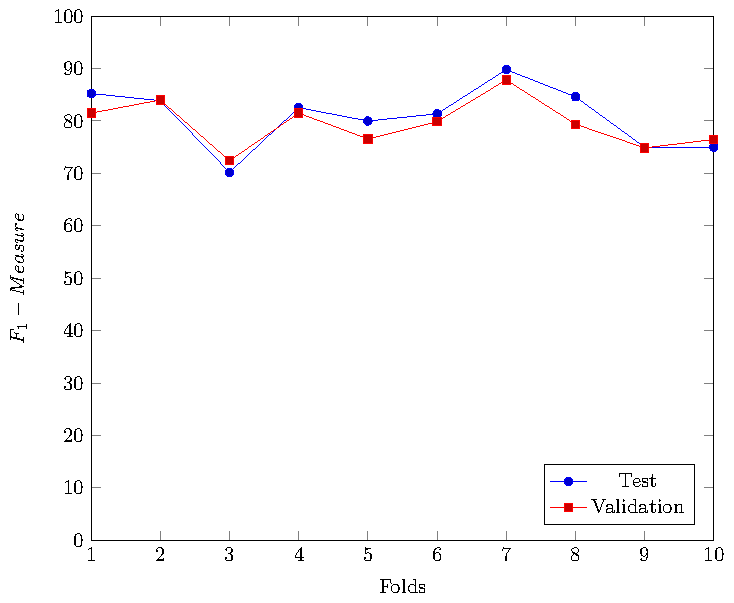
\includegraphics[width=\textwidth]{img/prai/siamese_test_validation/siamese_test_validation}
		\caption[]%
		{{\small Siamese Network}}    
		\label{fig:siamese_val_test}
	\end{subfigure}
	\caption[  ]
	{$ F_1 -Measure$ in validation and test achieved by the 4 methods in each folds} 
	\label{fig:score_val_test}
\end{figure}
\begin{figure}
	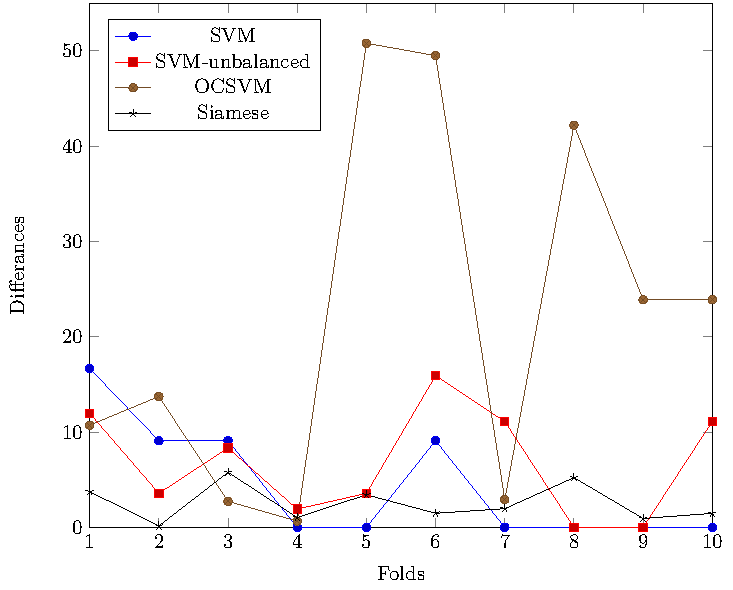
\includegraphics[width=\linewidth]{img/prai/diff_test_validation/diff_test_validation}
	\caption{Absolute value of differences between the validation and test $ F_1 -Measure$ for each fold}
	\label{fig:diff_test_validation}
\end{figure}
\begin{table}[ht]
	%	\caption{Best hyper-parameters find in random-search phase for Siamese network\tablefootnote{Value in the square brackets represents the value adopted for each layer.}.}\label{tab:opt_hyperparam}
	\caption{Best hyper-parameters find in random-search phase for Siamese network\protect\footnotemark[6].}\label{tab:opt_hyperparam}
	\centering
	
	\begin{tabular} {c | c}
		\hline
		\textbf{Parameter} 		& \textbf{Value} \\  
		\hline
		Cnn layer Nr. 	& 4		                          \\
		\hline
		Kernel shape 	& [[3x3],[3x3],[3x3],[3x3]]     \\
		\hline									
		Kernel Nr. 		& [32,32,32,32]	                            \\
		\hline   
		Stride & [[1x1],[1x1],[1x1],[1x1]]			                          \\
		\hline
		Dilation & [[1x1],[1x1],[1x1],[1x1]]  \\
		\hline
		Max pool shape & [[2x1],[1x3],[1x2],[3x2]]     \\
		\hline                   
		MLP layers Nr. 	&	3	                          \\
		\hline
		MLP layers dim.	& [3000,300,30]                        \\
		\hline
		Batch size	&	[100]                                    						\\
		\hline 
		Dropout & [Yes]        \\
		\hline
		Drop rate	&	[0.5]                         \\
		\hline
		Learning rate decay	&	[$0.1$] \% \\
		\hline                
		Batch normalization	&	[yes,no,no,no,yes,yes,yes]                   \\
		\hline
		
	\end{tabular}
\end{table}


The Siamese Network seems to be promising. Without the needing of humans falls for training, it can reduce to zero the miss rate showing also a good generalization performance with respect to the others methods. All these elements suggest that it can be used in a real scenario, but it has to be assessed also in others conditions.
In \secref{sec:siamese_one_shot}, a method based on this work will be evaluated inserting in the test even more types of audio events and noises.
Another interesting evaluation, as future work, could be to evaluate how the system behaves if trained on different data sets with respect to the one used here, also using transfer learning techniques. This is important because it could relax the necessity of carrying out a data collection campaign in every environment in which the system is going to be installed. In addition, other types of networks such as Recurrent Neural Networks or Long Short-Term Memory that have not been explored in this work could be tested.




\section{Audio Metric Learning by using Siamese Autoencoders for One-Shot Human Fall Detection}
\label{sec:siamese_one_shot}

As aforementioned, the fall detection task is very challenging due to the difficulty in retrieving examples for human fall modeling. Falls simulated by using a dummy may not represent properly real human falls, because they can not recreate falls in which arms are used to mitigate the impact. Moreover, the use of protections, such as mattresses, knee pads or foam during the acquisitions of falls performed by volunteers, can significantly modify the samples, especially in the audio field. 
We assess our proposed method in a complex scenario. The whole dataset described in \secref{sec:dataset} has been used.
Moreover, an innovative Siamese approach for fall detection, that exploits the similarities between simulated and real human falls by using only one \textit{RHF} template per each room during training into a one-shot learning perspective is proposed.
In order to do this, we used a Siamese Autoencoder (SAE) for metric learning. Selecting the pairs appropriately for training the SAE, the network learns how to map simulated falls to real falls applying a transformation directly into the embedding space. After that, we use the encoder part of the whole network to create new human fall templates by using simulated falls. Concluding, a classifier is trained by using the new synthetic templates in addiction with the real fall templates to discriminate between fall and non-fall event.
As shown in \secref{sec:soa}, although the literature provides several supervised and unsupervised approaches, no solution has been proposed exploiting one-shot learning for fall detection, nor to fill the gap between simulated falls and scarcely available real human falls.


\subsection{Dataset}
The dataset used here in an extension of the dataset used in all our previous works that was created specially for this work: the new recordings have been performed in 2 different rooms (R1 and R2) with respect to the original one. Each room has different characteristics that make the propagation of waves less favorable: one room is paved with a fitted carpet floor, while in the other, the FAS was placed beyond a soundproof wall and the floor is made of stoneware tile. We also recorded other objects and background types in addition to those present in the previous dataset. Here the human falls were reproduced by volunteers without additional protections. Only the signals recorded with FAS has been used in this work. For a more detailed description, refer to the dedicated \secref{sec:dataset} and \tableref{tab:numDataset}.
This complete dataset allows a more exhaustive experimental evaluation of the Siamese approach highlighting its effectiveness in a one-shot learning framework with respect to other state-of-the-art methods.

\subsection{Proposed Method}
The proposed fall classification system is composed of 3 main parts described in this section.
First, the features are extracted from row audio file and later used to train a Siamese neural network for metric learning. At the end a metric-based classifier is used to discriminate human falls from non-human falls.

\subsubsection{Feature Extraction Stage}
In the feature extraction stage, the raw audio signals have been preprocessed to compute the log mel-energies, thus obtaining a 2D matrix representing the samples.
Such features have been chosen for their popularity in computational audio analysis \cite{gemmeke2013exemplar, mesaros2010acoustic, parascandolo2017convolutional}.

\subsubsection{Metric Learning Stage}
The second block is a nonlinear metric learning stage based on Siamese Neural Network (SNN). The SNN is directly trained on semantic similarity information, that aims at modeling the relationships between classes in order to extract more robust features. The proficiency of a SNN mostly depends on the objective function used to train the network as well as the training set selection strategy. Our contribution consists in defining these two aspects. 
\begin{figure*}
	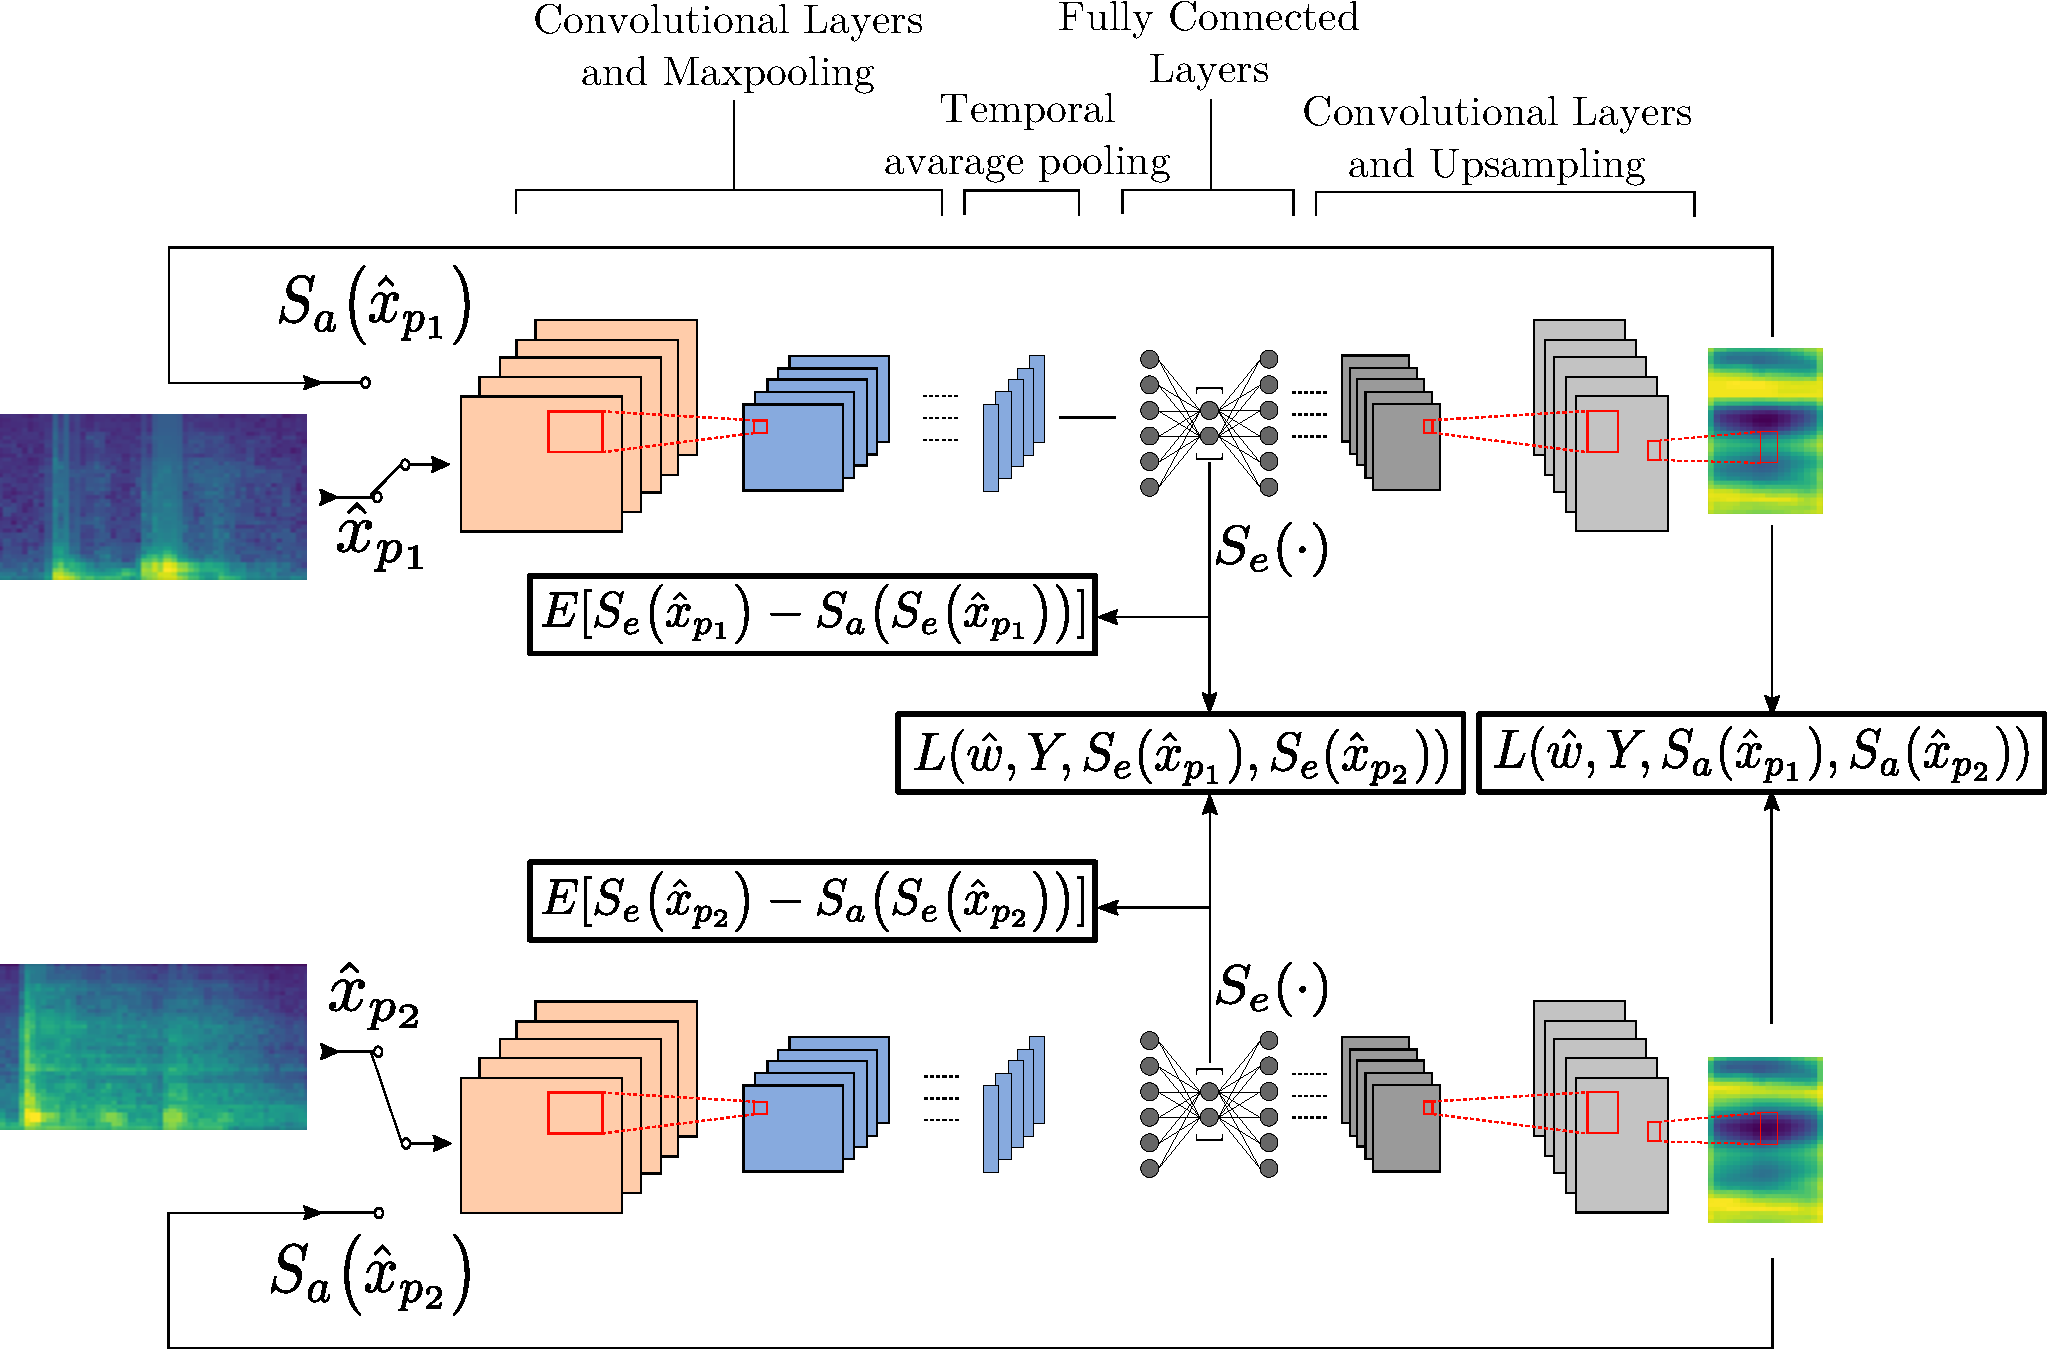
\includegraphics[width=\linewidth]{img/eeai/Siamese_approach}
	\caption{The architecture of the SCAE network for metric learning and robust feature extraction. The loss terms used for training the network are shown.}
	\label{fig:proposed_approach}
	
\end{figure*}
The proposed neural network architecture, depicted in \figref{fig:proposed_approach}, consists in a Siamese Convolutional Autoencoder (SCAE). This is composed by an encoder that applies a transformation of the input into the latent space and a decoder that performs the reverse operation. The encoder includes some convolutional layers alternated - in some configurations - with max-pooling layers, followed by some fully connected layers. The encoder ends with a hidden layer representing the mapping of the inputs. Before the fully connected layers, average pooling is applied along the time dimension of the features map related to the last convolutional layer. This makes the network independent from the temporal length of the input signals. The decoder part is mirrored with respect to the encoder. 
Our Siamese Neural Network is devoted to learning a projection metric in a weakly-supervised way from input pairs in the form of positive and negative examples: 	

\begin{equation}
\label{eq:positive}
\mathcal{P} = \{(\hat{x}_{p_1}, \hat{x}_{p_2} ) : \hat{x}_{p_1} \textrm{ and } \hat{x}_{p_2} \textrm{come from same distribution}\},
\end{equation}
\begin{equation}
\label{eq:negative}
\mathcal{N} = \{(\hat{x}_{p_1}, \hat{x}_{p_2} ) : \hat{x}_{p_1} \textrm{ and }  \hat{x}_{p_2} \textrm{come from different distributions}\}
\end{equation}
%\begin{center}
%	$\mathcal{P}$ = \{($\hat{x}_{p_1}$, $\hat{x}_{p_2}$ ) : $\hat{x}_{p_1}$ and  $\hat{x}_{p_2}$ come from same distribution\}, \\
%	$\mathcal{N}$ = \{($\hat{x}_{p_1}$, $\hat{x}_{p_2}$ ) : $\hat{x}_{p_1}$ and  $\hat{x}_{p_2}$ come from different distributions\}. 
%\end{center}
with $\hat{x}_{p_1}$ and $\hat{x}_{p_2}$ the first and second input of the SCAE respectively.
Considering $Y(\hat{x}_{p_1}, \hat{x}_{p_2})$ as the label assigned to the pair, training consists in finding a set of weights $\hat{w}$ that minimizes, for each input pair, the contrastive loss function defined as 
\begin{equation}
L(Y, S_e^w(\hat{x}_{p_1}),  S_e^w( \hat{x}_{p_2})) = (1 - Y)\frac{1}{2}(E_w)^2 + (Y)\frac{1}{2}\{(max(0, m - E_w)\}^2,
\end{equation}
with 
\begin{equation}
E_w = \norm{S_e^w (\hat{x}_{p_1}) - S_e^w (\hat{x}_{p_1})}.
\end{equation}
the Euclidean distance between the two mappings performed by the encoder and $S_e^w(x_p)$ the actual encoder function.
To strengthen the metric learning, the decoder part of the network has been used to add two more terms to the loss function. The first is the contrastive loss function between the two signals reconstructed at the end of the autoencoder, that is $S_a^w(\hat{x}_{p_1})$ and $S_a^w(\hat{x}_{p_2})$. This is possible thanks to the average pooling layer previously mentioned. In fact, with this layer the autoencoder reconstructs a signal with fixed time length, regardless of the length of the input signals, allowing the Euclidean distance between the two reconstructions to be computed. Without the temporal average pooling layer, the reconstructed zero padded part of the input signals would control the value of the Euclidean distance, invalidating the result and leading to incorrect training. The typical capability of an autoencoder to exactly reconstruct the input signal is now lost. This is a fundamental feature that forces the autoencoder to engage in robust feature learning. Since it is impossible to add this term in a standard way due to the different dimensions between input $\hat{x}_{p}$ and reconstructed input $S_a^w(\hat{x}_{p})$, the network has been forced to rebuild the latent layers of the input $S_e^w(\hat{x}_{p})$ and the reconstructed signal $S_e^w(S_a^w(\hat{x}_{p}))$ by adding the following Mean Squared Error terms to the loss:

\begin{equation}
E [ S_e \big(\hat{x}_{p_2}\big) -  S_a \big(S_e \big(\hat{x}_{p_2}\big)\big)].
\end{equation}

As mentioned previously, another crucial aspect of SNN is the selection of training pairs.
Since we are creating a fall detection system that uses as few examples of \textit{RHF} as possible, it is necessary to take full advantage of the limited information available. Moreover, since examples of simulated falls are available, the similarities between these two types of fall must be exploited. In order to do this, the training set for the SCAE was created by combining the following signals:
\begin{itemize}
	\item to compose the negative set $\mathcal{N}$, all classes of objects available in the dataset and background noises have been used. No real or simulated human falls have been coupled with other sounds;
	\item all classes available in the dataset has been used to compose the positive set $\mathcal{P}$.
\end{itemize}
%The idea is to let the network map the real and simulated falls where it wants, clearly based on how the other classes are mapped. The only constraint is to make them similar to each other in the embedding representation of the autoencoder. This allows the network to learn, during the training, to make a transformation of human falls directly into the latent space. For further details, please refer to \secref{sec:preliminary_experiments}.
The idea is to let the network map the real and simulated without particular constraints, in order to identify the hyper-space region where the \textit{RHF} of the test set will be mapped. The only restriction is to make them similar to each other in the embedding representation of the autoencoder. This allows the network to learn, during the training, to make a transformation of human falls directly into the latent space. For further details, please refer to \secref{sec:preliminary_experiments}.

\subsubsection{Classification Stage}
\label{sec:classification_stage}
In the end, the resulting function is used to improve the performance of metric-based classifier that discriminates falls from non-falls.
All the train set is first transformed using the encoder function $S_e^w(\cdot)$. Moreover, we apply this transformation also to some instances of \textit{SHF} previously left out of the train set of the SCAE, thus obtaining a total number of templates for the human fall equal to 
\begin{equation}
\mathcal{T}_{hf} = \mathcal{T}_{shf} + \mathcal{T}_{rhf},
\end{equation}
with $\mathcal{T}_{shf}$ the number of \textit{SHF} from R0 and $\mathcal{T}_{rhf}$ the total number of \textit{RHF} templates selected from R1 and R2 used in SCAE training, two in our case. To train the \textit{knn} classifier, a set of templates composed of $\mathcal{T}_{hf}$ instances have been selected for each other class in order to obtain a balanced training set. Besides, the parameter \textit{K} of the classifier has been set to $\mathcal{T}_{hf}$. Finally, a human fall is detected if there is at least one human fall template in the set of $\mathcal{T}_{hf}$ neighbors related to the sample under test at that moment. This classification technique has been used to reduce to a minimum the miss rate which, for this particular application, have a greater weight compared to false alarm rate.

\section{Comparative methods}
In this section, the methods compared with the proposed work are summarized.
The first method is based on a bi-class Support Vector Machine. It uses a mixture of gaussians (GMM), trained on a large corpus of audio events with the Expectation Maximization algorithm to model the acoustic space (Universal Background Model, UBM). Then, for each audio segment, the Maximum a Posteriori (MAP) algorithm is used to calculate the Gaussian Mean Supervector (GMS) from the MFCCs. Please refer to \secref{sec:biclass_svm} for further details. This method will be shown in 2 variants, the first (SVM from now on) with a balanced train set, while the second (One-shot-SVM from now on) with an unbalanced train set for direct comparison with the proposed approach.
The second is the unsupervised variation of the previous one based on OCSVM (\secref{sec:ocsvm_approach}).
The third is the method that has been extended in this work, presented in \secref{sec:siamese_few_shot} and named \textit{Original Siamese} from now on. It consists of a simple SNN instead of SCAE thus equivalent to the encoded part of the proposed autoencoder architecture, but without the average pooling layer before the fully connected layers. In \secref{sec:siamese_few_shot} the algorithm worked in a more facilitated scenario as several human falls were used during training. Hear instead we perform the method in a one-shot learning framework. Since dummy-like falls were not used in this method, the pairs generation technique consists in the combination of the non-human fall data and the available template of \textit{RHF} in order to compose the positive $\mathcal{P}$ and negative $\mathcal{N}$ as indicated in \equationref{eq:positive} and \equationref{eq:negative}. Furthermore, a threshold based classifier is used. A human fall is detected if the sample is mapped within a radius from a real human fall template.

\subsection{Experiments}
This section presents, first, how data was selected for each compared methods. Then, an in-depth analysis of the preliminary experiments is discussed to gain insights on the behavior of the proposed approach and some of its variant. In the end, the classification performances of the optimized algorithms are reported. 
All the experiments have been assessed on the dataset described in \secref{sec:dataset}, but signals have been downsampled to 8\,kHz and the resolution has been reduced to 16\,bits.
All the following experiments have been conducted with 120000 pairs, on average between folds, for training the SCAE. Results are expressed in terms of F$_1$-Measure, calculated from the normalized confusion matrix, cumulative of all the folds. The same metric has also been used to optimize the results shown in \secref{sec:opt_results}. This choice was made to give more weight to false negatives than false positives, as the test set is highly unbalanced, being composed from 6973 non-human fall events and 390 human fall events in total. In particular, since the background tracks have been divided into segments of 5 seconds each, the non-fall events are composed of 5275 background instances and 1698 object fall events.

\subsubsection{Data Splitting}

Firstly, dataset has been split into 5 folds for cross-validation: in particular, the data related to R0 room, except for \textit{SHF}, have been used only for training and used in each fold. Differently, the samples related to R1 and R2, except for \textit{RHF}, have been split into 5 folds with 20\% for test and 80\% for the training set. Both simulated and real human falls have been treated differently, based on the algorithm under examination:
\begin{itemize}
	\item SCAE: for the proposed approach, one \textit{RHF} per room has been randomly selected for each fold and then added to the related trainset. The \textit{SHF}, instead, have been split in 5 folds with 80\% for train the SCAE, while the remaining 20\% has been left out from the training set of the Siamese network but used only to train the classifier as explained in  \secref{sec:classification_stage}. The pairs for training the SNN have been generated keeping balanced all the combinations between the classes.
	\item OCSVM: since this is a completely unsupervised method, both real an simulated human falls have been removed from trainset.
	\item SVM: since this is a completely supervised method, the \textit{RHF} have been split in 5 folds with 20\% for test and 80\% for train and then added to the respective sets. 
	\item One-shot-SVM: in order to keep this experiment comparable with the proposed method, the same selection carried out for the SCAE has been used for train the SVM, i.e. with just one real human fall sample for each environment to monitor. 
	\item \textit{Original Siamese}: the same lists used for SCAE have also been used for this approach. The only difference is that the \textit{SHF} were not used because are not contemplated by this method.
	
\end{itemize}

\subsubsection{Preliminary Experiments}
\label{sec:preliminary_experiments}
Before running the optimization phase, the behavior of different pairs generation techniques for SCAE training has been studied. To do this, 4 preliminary experiments have been performed with a fixed autoencoder architecture, that has a hidden layer composed of just 2 neurons in order to visualize how the system maps the input signals when varying the way in which real and simulated falls are paired. \tableref{tab:preliminary_network} reports the hyper-parameter of that network. In \figref{fig:p-n-pairs}, \figref{fig:n-pairs}, \figref{fig:no-pairs} and \figref{fig:p-pairs} it can be seen how training and testing signals are encoded by the network, after its training, in the 4 different cases named $\mathcal{P}$-$\mathcal{N}$-PAIRS, $\mathcal{N}$-PAIRS, NO-PAIRS and $\mathcal{P}$-PAIRS  .
The mappings in \figref{fig:train-p-n-pairs}, \figref{fig:train-n-pairs}, \figref{fig:train-no-pairs} and \figref{fig:train-p-pairs} are then used to train the related \textit{knn} classifier, following what was said in section \secref{sec:classification_stage}. The final decision boundaries are reported in all figures: the data found in the white area are classified as human fall. Moreover, the \textit{RHF} have been highlighted with orange stars while \textit{SHF} with green X. The turquoise X instead, represent the encoded \textit{SHF} previously left out from the SCAE trainset, but then added to the train set of the \textit{knn} classifier.
The 4 strategies for generating the pairs containing \textit{RHF} and/or \textit{SHF} are described below:
\begin{itemize}
	\item $\mathcal{P}$-$\mathcal{N}$-PAIRS (\figref{fig:p-n-pairs}): the \textit{RHF} and \textit{SHF} were joined together to form positive examples and with other signals to form negative examples. In this case, it can be observed how the network manages to separate the signals of human falls well during training. However, this is not generalized on the test set where the \textit{RHF} are mapped to a different area. This means that the knowledge of a few human falls is not exploited properly. 
	\item $\mathcal{N}$-PAIRS (\figref{fig:n-pairs}): the human fall-related instances have been coupled only with signals of different classes, thus obtaining only a subset to add to the negative examples set. As it can be seen from \figref{fig:train-n-pairs}, in this case, the contrastive loss tries to repulse the human fall instances from everything else, but without grouping them together (no positive examples were generated).
	%    Although this happens for the simulated falls, the few instances of pairs containing a real fall in the train set of the Siamese network are not enough for this removal.
	This results in poor classification performance as shown in \tableref{tab:preliminary_resuts}.
	Moreover, in both the $\mathcal{P}$-$\mathcal{N}$-PAIRS and $\mathcal{N}$-PAIRS methods, the usage of \textit{SHF} seems not useful.
	\item NO-PAIRS (\figref{fig:no-pairs}): neither \textit{RHF} nor \textit{SHF} were used for the training of the SCAE, but only for the training of the classifier. In this situation, the SCAE spreads the simulated human fall signals in the hyperplane (\figref{fig:train-no-pairs}) that, when used to train the classifier, leads to the generation of too many false alarms as can be observed in \figref{fig:test-no-pairs}. 
	\item $\mathcal{P}$-PAIRS (\figref{fig:p-pairs}): is best performing strategy. In this case, the human fall-related instances have been coupled only together, thus obtaining only a subset to add to the positive examples set. In this way, the SCAE is free to map human falls (both real and simulated) in the zone of space it wants, but keeping them close to each other. In this way, the network learns to transfer the features of the real falls to the simulated falls directly in the latent space. Now the \textit{SHF} left out of the SCAE training can be used as additional templates for training the \textit{knn} classifier.
\end{itemize}
The results for these preliminary experiments are reported in \tableref{tab:preliminary_resuts}, where can be observed the best performance obtained with the fourth pairs generation strategy.
\begin{table}[t]
	\caption{Hyper-parameters used in the preliminary experiments, and their value}
	\label{tab:preliminary_network}
	\centering
	\footnotesize
	\begin{tabular} {|c | c|| c | c|}
		\hline
		Parameter 		& Range &Parameter & Range \\  
		\hline\hline
		CNN layer Nr. 	& 3 & Drop rate & 0\% \\
		\hline
		Kernel shape 	& [4x4,4x4,4x4]& CNN Padding	& same  \\
		\hline									
		Kernel Nr. 		& [4,4,4]&Batch Size&	512 \\
		\hline                                     
		MLP layers Nr. 	& [3] & MLP Act.&	ReLU\tablefootnote{In the decoder, an additional Cnn layer with $tanh$ activation function has been used to ensure a good reconstruction.} \\
		\hline
		MLP layers dim.	&[40,512,2]\% & Optimizers 	& Adadelta	 \\
		\hline
		Max pool shape & [1x2,2x3,2x3] & Weight Initializers & Glorot Uniform	 \\
		\hline
	\end{tabular}
\end{table}	

\begin{table}[t]
	\caption{Preliminary result for different pairs generation strategies.}
	\label{tab:preliminary_resuts}
	\begin{center}
		\begin{tabular}[t]{|c||c|c|c|}
			
			\hline
			\textbf{Technique} & \textbf{Result in R1} & \textbf{Result in R2} & \textbf{Overall} \\ %\cline{2-5} 
			\hline
			$\mathcal{P}$-$\mathcal{N}$-PAIRS      				& 55.17\%    &   64.74\% 	&   60.13\%   	\\
			$\mathcal{N}$-PAIRS       			& 76.20\%    &   67.53\% 	&   72.05\%     \\
			NO-PAIRS     				& 91.71\%    &   89.88\%	&   90.97\%    	\\
			$\boldsymbol{\mathcal{P}}$\textbf{-PAIRS}       	& 92.54\%    &   92.54\%	&   \textbf{92.54\%}    	\\
			\hline
		\end{tabular}
	\end{center}
\end{table}
\begin{figure*}[h!]
	\centering
	\begin{subfigure}[b]{0.475\textwidth}   
		\centering 
		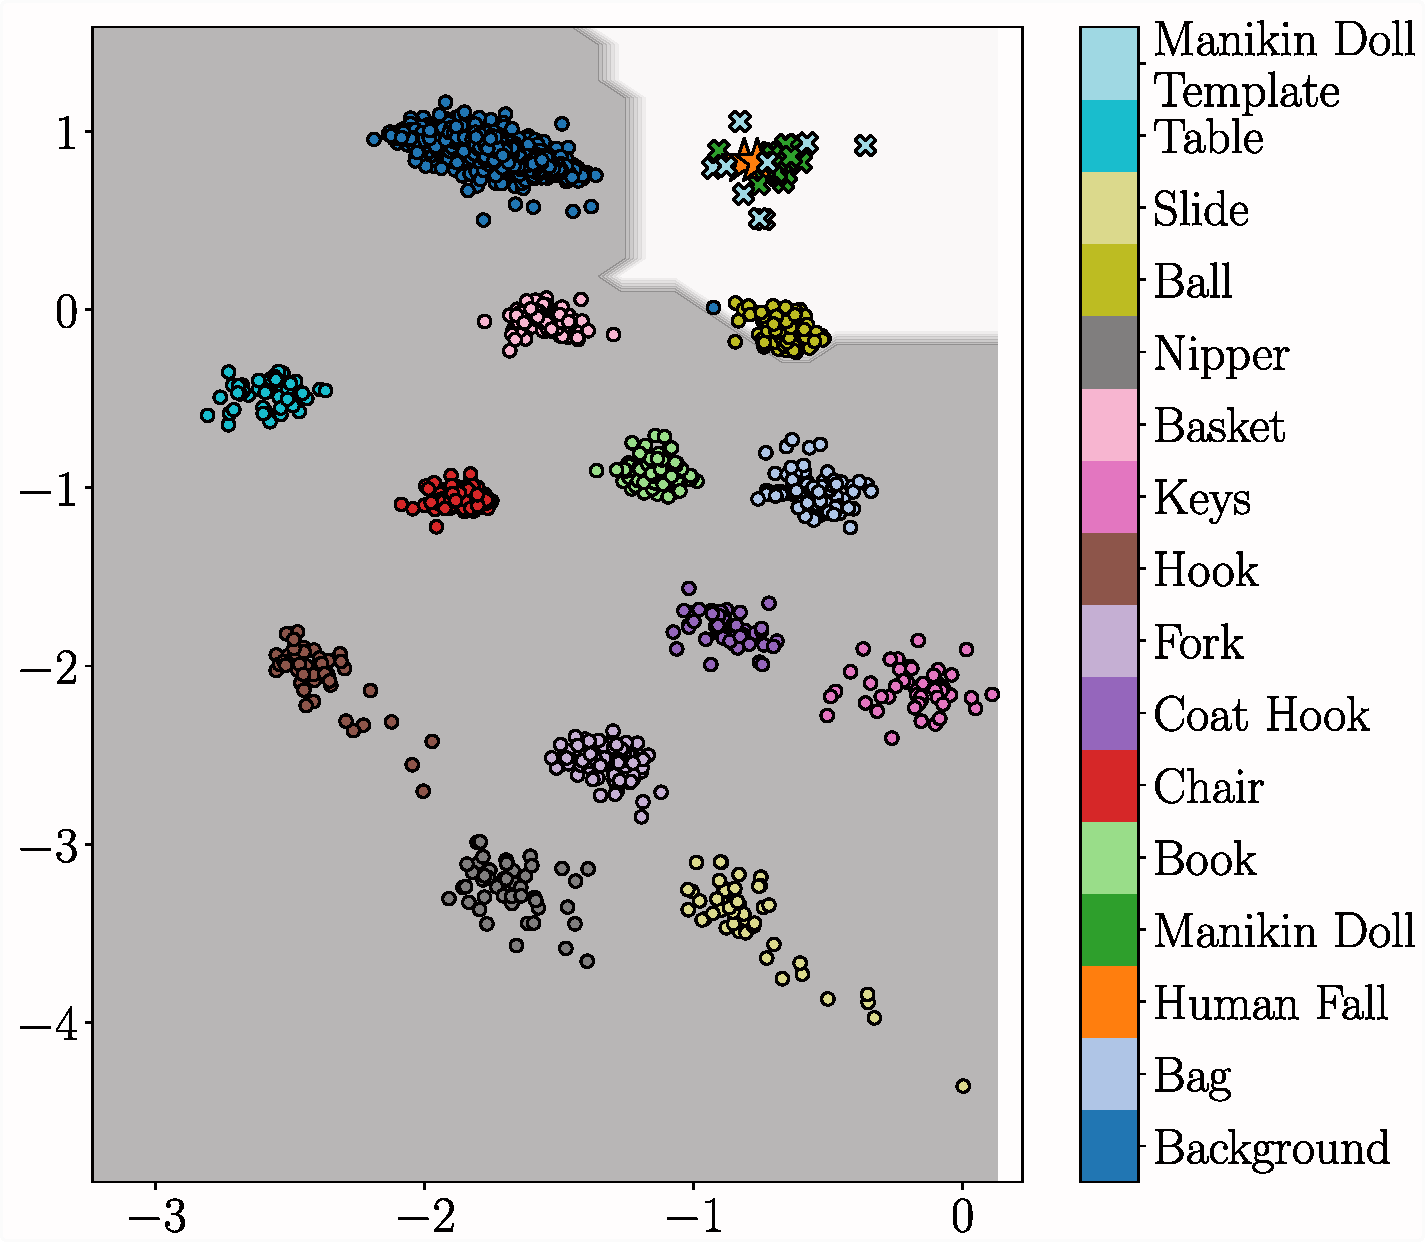
\includegraphics[width=\textwidth]{img/eeai/embedding/positive_negative_template_pairs/fold_2_train}
		\caption[]%
		{\small Training set.}    
		\label{fig:train-p-n-pairs}
	\end{subfigure}
	\quad
	\begin{subfigure}[b]{0.475\textwidth}   
		\centering 
		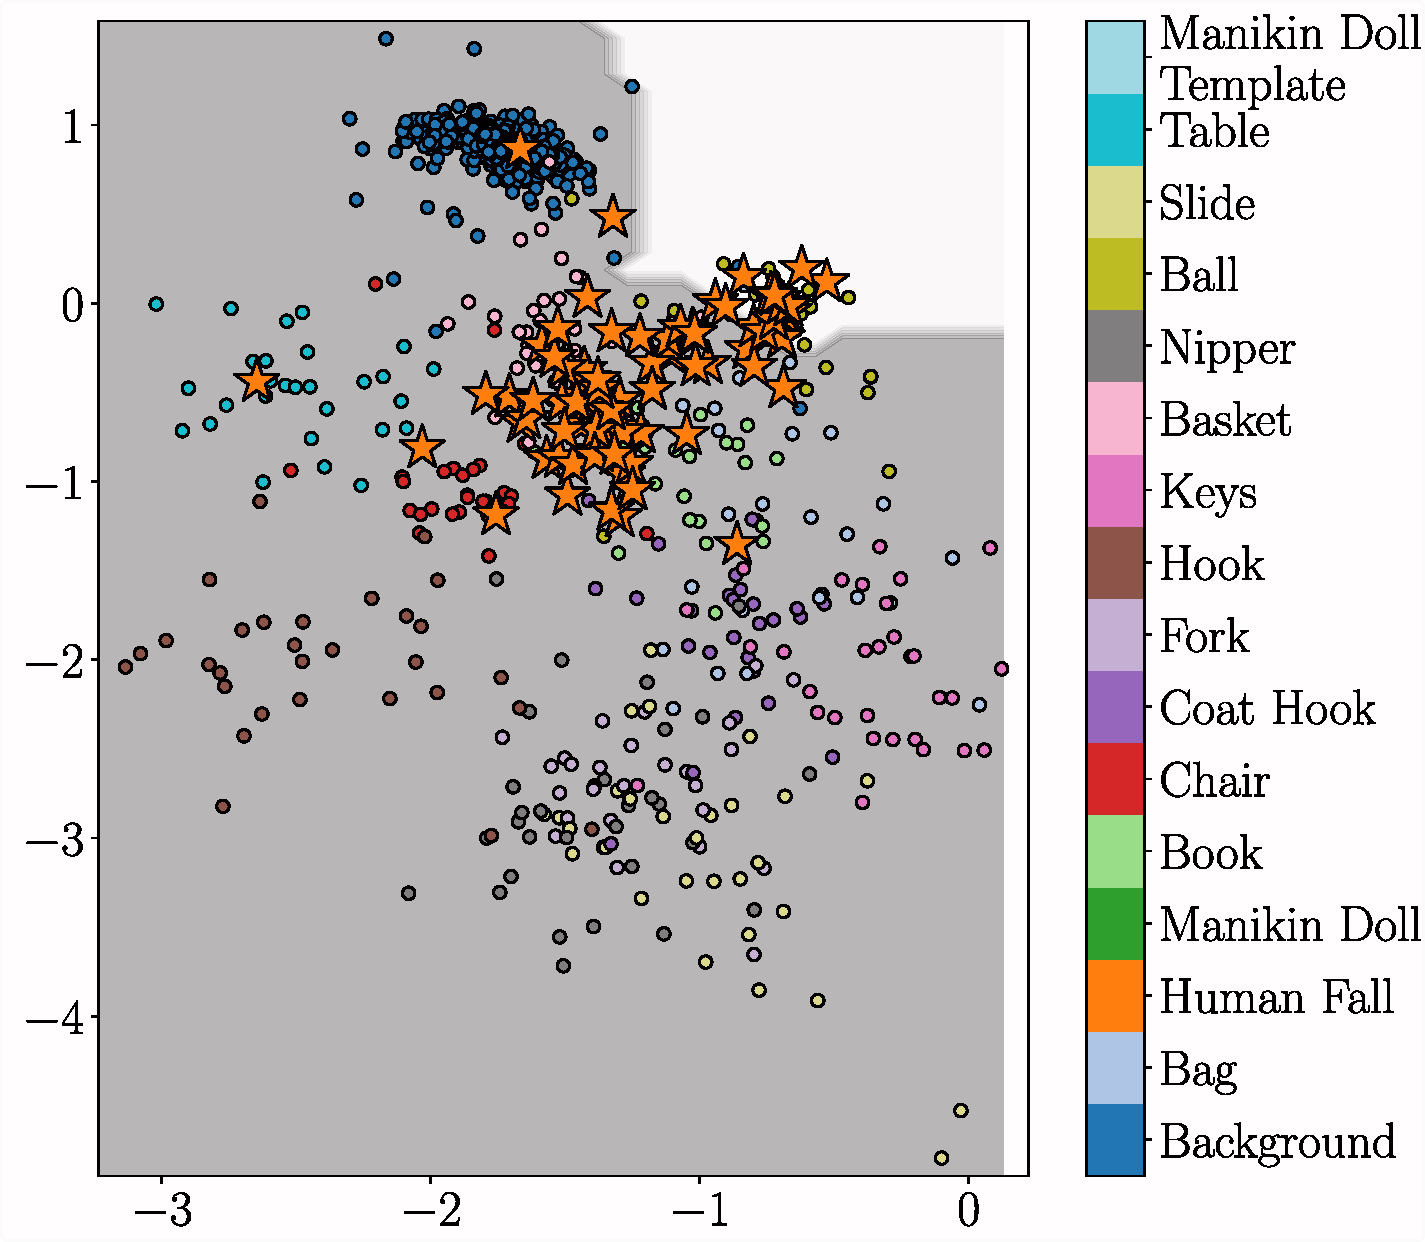
\includegraphics[width=\textwidth]{img/eeai/embedding/positive_negative_template_pairs/fold_2_moquette}
		\caption[]%
		{ Test set.}    
		\label{fig:test-p-n-pairs}
	\end{subfigure}
	\caption[]
	{\small Two-dimensional embedding performed by the encoder function $S_e^w(\hat{x}_{p})$ with $\mathcal{P}$-$\mathcal{N}$-PAIRS strategy.} 
	\label{fig:p-n-pairs}
\end{figure*}
\begin{figure*}[h!]
	\centering
	\begin{subfigure}[b]{0.475\textwidth}   
		\centering 
		\includegraphics[width=\textwidth]{img/eeai/embedding/negative_template_pairs_only/fold_4_train}
		\caption[]%
		{Training set}    
		\label{fig:train-n-pairs}
	\end{subfigure}
	\quad
	\begin{subfigure}[b]{0.475\textwidth}   
		\centering 
		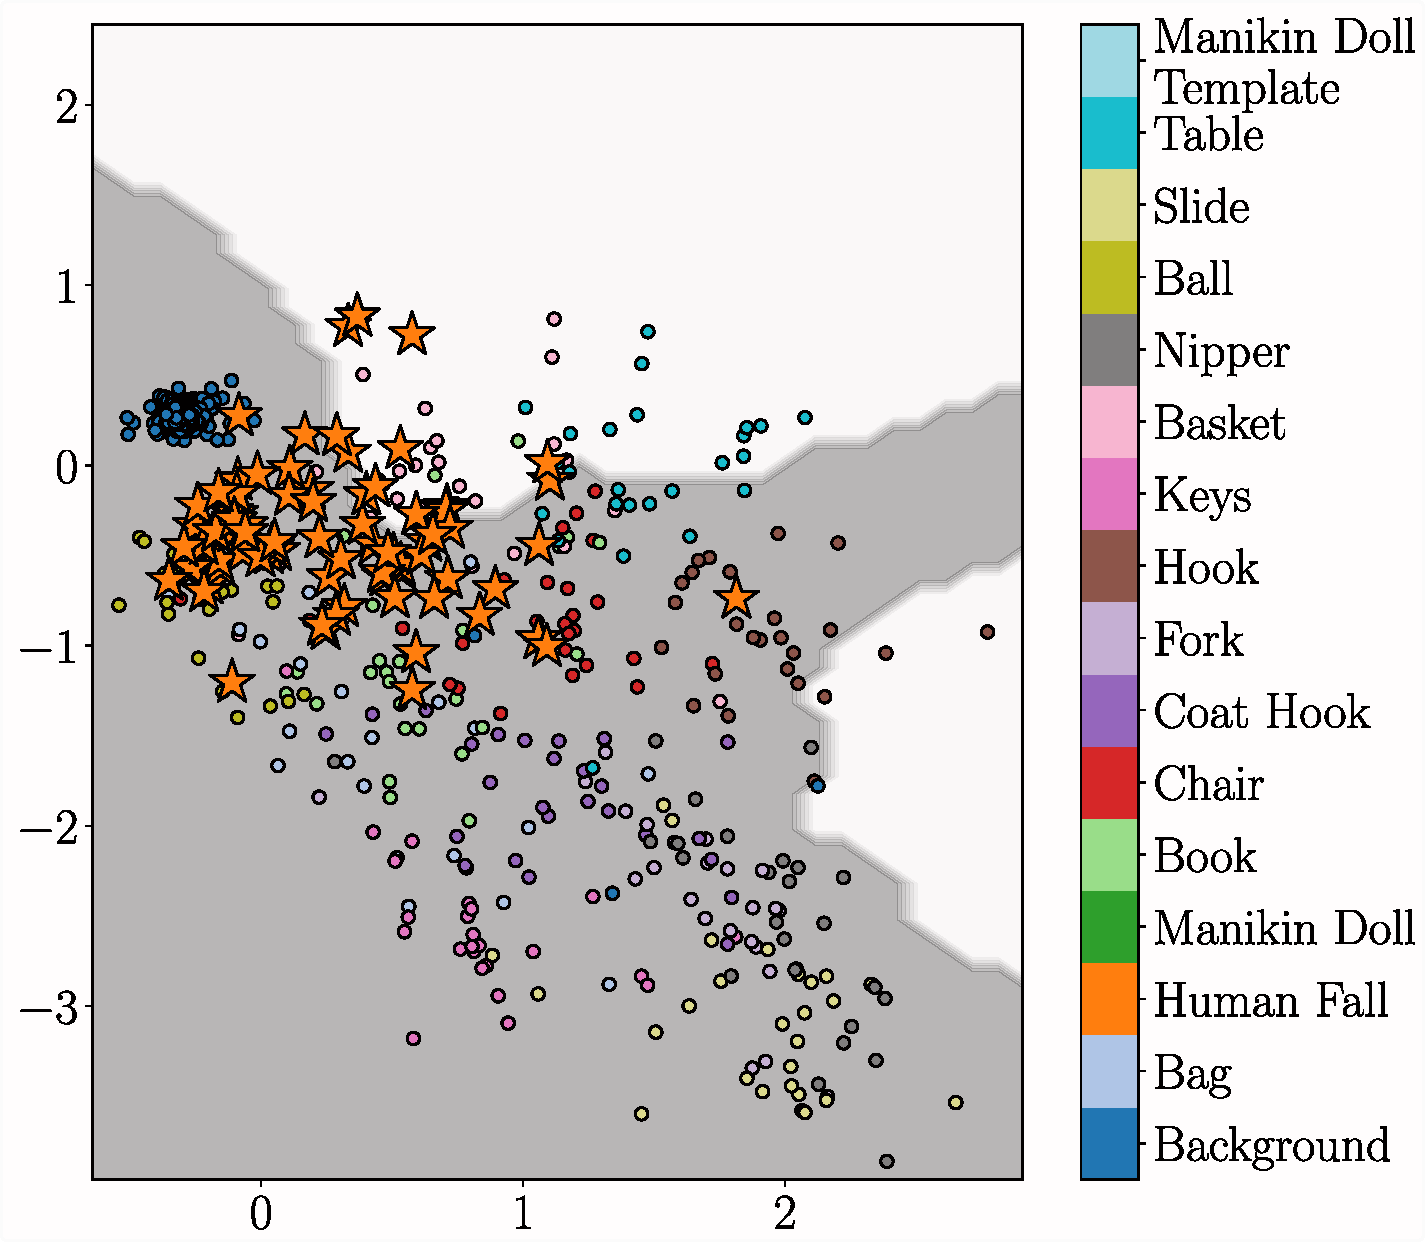
\includegraphics[width=\textwidth]{img/eeai/embedding/negative_template_pairs_only/fold_4_moquette}
		\caption[]%
		{Test set}    
		\label{fig:test-n-pairs}
	\end{subfigure}
	\caption[]
	{\small Two-dimensional embedding performed by the encoder function $S_e^w(\hat{x}_{p})$ with $\mathcal{N}$-PAIRS strategy} 
	\label{fig:n-pairs}
\end{figure*}

\begin{figure*}[h!]
	\centering
	\begin{subfigure}[b]{0.475\textwidth}
		\centering
		\includegraphics[width=\textwidth]{img/eeai/embedding/no_template_pairs/fold_4_train}
		\caption[]%
		{Training set.}    
		\label{fig:train-no-pairs}
	\end{subfigure}
	\hfill
	\begin{subfigure}[b]{0.475\textwidth}  
		\centering 
		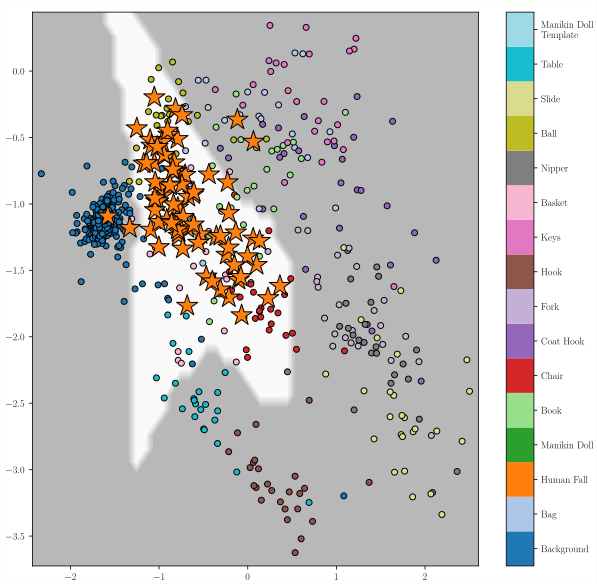
\includegraphics[width=\textwidth]{img/eeai/embedding/no_template_pairs/fold_4_moquette}
		\caption[]%
		{Test set.}    
		\label{fig:test-no-pairs}
	\end{subfigure}
	\caption[]
	{\small Two-dimensional embedding performed by the encoder function $S_e^w(\hat{x}_{p})$ NO-PAIRS strategy.} 
	\label{fig:no-pairs}
\end{figure*}

\begin{figure*}[h!]
	\centering
	\begin{subfigure}[b]{0.475\textwidth}   
		\centering 
		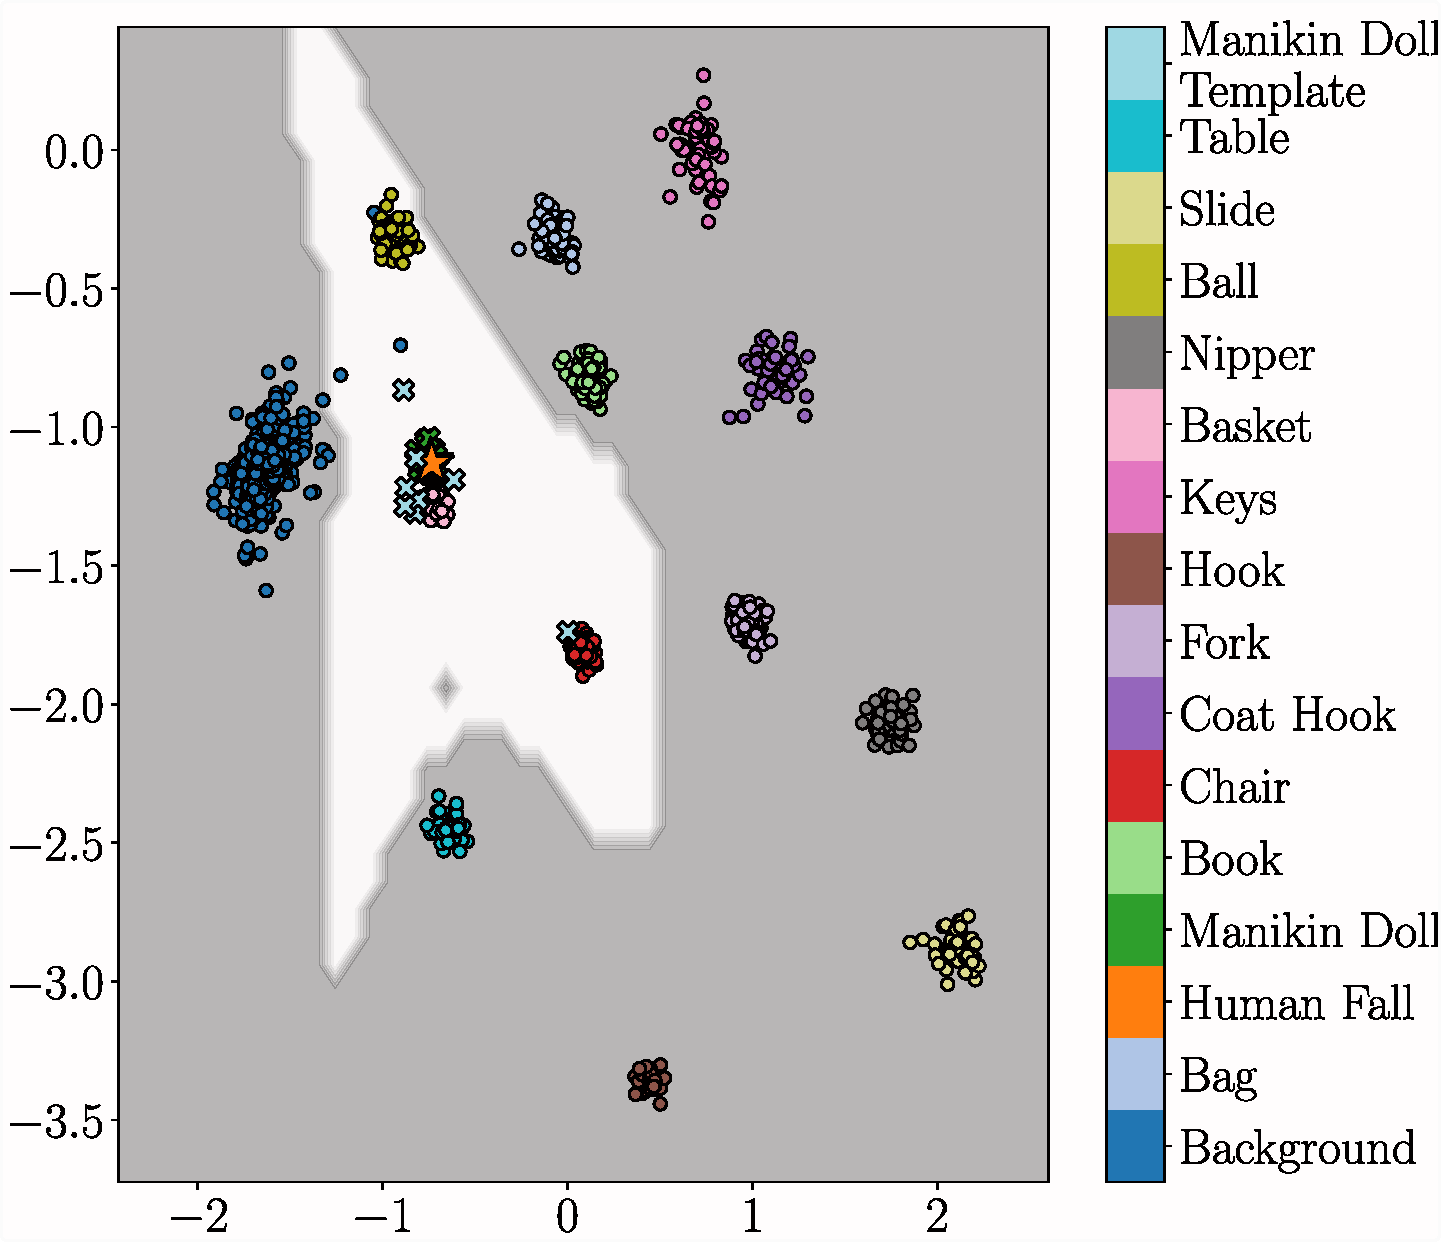
\includegraphics[width=\textwidth]{img/eeai/embedding/positive_template_pairs_only/fold_4_train}
		\caption[]%
		{Training set.}    
		\label{fig:train-p-pairs}
	\end{subfigure}
	\quad
	\begin{subfigure}[b]{0.475\textwidth}   
		\centering 
		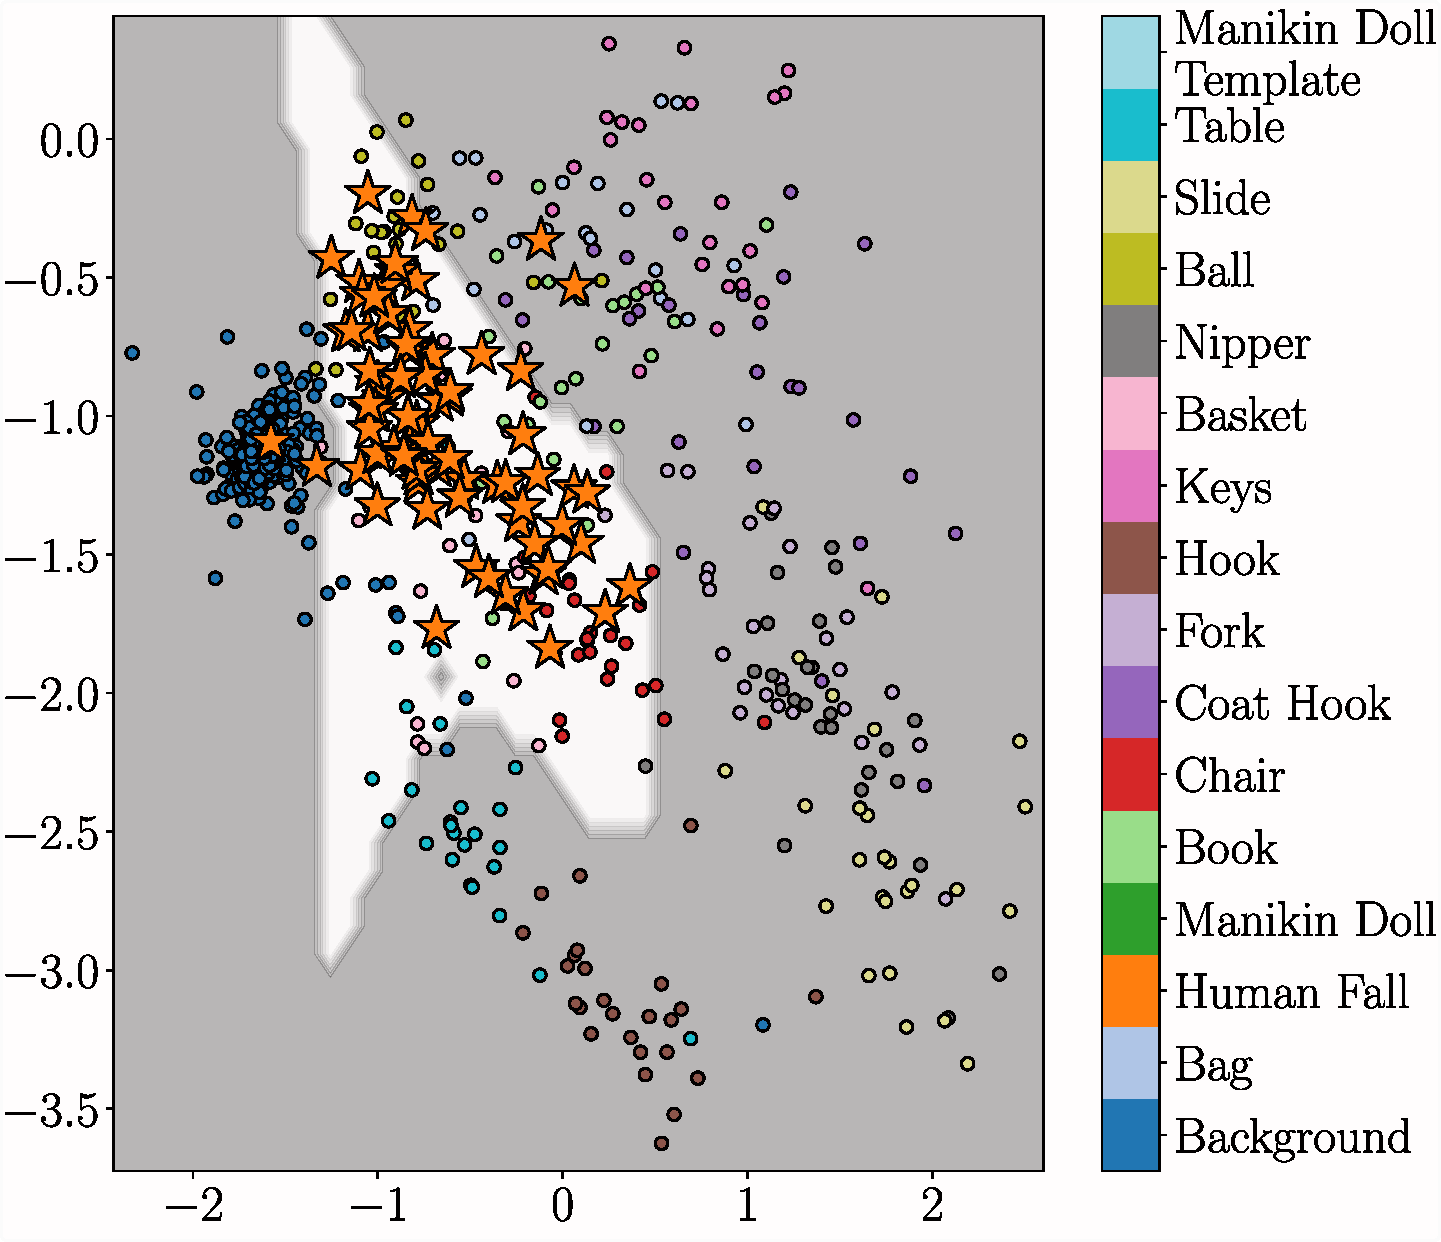
\includegraphics[width=\textwidth]{img/eeai/embedding/positive_template_pairs_only/fold_4_moquette}
		\caption[]%
		{Test set.}    
		\label{fig:test-p-pairs}
	\end{subfigure}
	\caption[]
	{\small Two-dimensional embedding performed by the encoder function $S_e^w(\hat{x}_{p})$ with $\mathcal{P}$-PAIRS strategy.} 
	\label{fig:p-pairs}
\end{figure*}


\subsection{Optimized results}
\label{sec:opt_results}
%l'svm non è dirrettamente comparabile a causa dei testset divero. Cmq il risultato evidenza quanto lo scenario in cui ci siamo posti possa essere complicato anche per approccio completamente supervised.
After observing the results of the preliminary experiments, a random-search of 50 different configurations was performed to optimize the hyper-parameters of the SCAE approach with the pairs generation strategy best performing in the preliminary experiments. At the end, we selected the configuration that reached the highest F$_1$-Measure in the test set. \tableref{tbl:hyper-params_few_shot} shows the value of the hyper-parameters used for network training and the relative search range. The unspecified parameters were left the same as those used in the preliminary experiments. The same random-search was also performed for the \textit{Original Siamese} method, also optimizing the radius of the classifier used with this approach. For the SVM based methods a grid-search strategy has been adopted to optimize the parameters. In particular the parameters have assumed values in the ranges  $\{ 2^{-5},2^{-3},\ldots,2^{15} \}$ for $ C $ (SVM) and $ \nu $ (OCSVM), $\{ 2^{-15},2^{-13},\ldots,2^{3} \}$ for $ \gamma $ (both SVM and OCSVM) and  $\{1,2,\ldots,64 \}$ for the number of mixtures of the GMM-UBM. 

\begin{table}[t]
	\caption{Hyper-parameters optimized in the random-search phase and their range.}
	\label{tbl:hyper-params_few_shot}
	\centering
	\footnotesize
	\begin{tabular} {|c | c | c|}
		\hline
		Parameter 		& Range & Distribution \\  
		\hline\hline
		Cnn layer Nr. 	& [1-3]& Uniform \\
		\hline
		Kernel shape 	& [1x1-8x8]& Uniform  \\
		\hline									
		Kernel Nr. 		& [1-32]& Uniform \\
		\hline                                     
		MLP layers Nr. 	&	[1-2]& Uniform \\
		\hline
		MLP layers dim.	&[1-4096]\% & Log-uniform \\
		\hline
		Max pool shape & [0x0-3x3] & Uniform\\
		\hline
		Drop rate &	[0-0.2]\% & Uniform	 \\
		\hline
	\end{tabular}
\end{table}																													
\figref{fig:results} shows the results obtained for each approach. Regarding the completely supervised SVM method, although it is not directly comparable with the others due to different training and test set, it gives an idea of how much the task is hard also for such a system. Moreover, using an extremely unbalanced dataset for a supervised approach, as the same used for the Siamese network, leads to a very marked decrease in performance. In fact, the One-Shot SVM reaches an overall F$_1$-Measure of only 14.72\%. When having an extremely unbalanced dataset available is better to use a completely unsupervised method such as OCSVM, that achieves a score of about 72\%. 
The best performing method is the SCAE that reaches a 93.58\% of F$_1$-Measure, outperforming the \textit{Original Siamese} of 3.25\%. The improvement was significant for p $<$ 0.002 according to one-tailed z-test \cite{smucker2007comparison}. The remarkable results obtained by both the \textit{Original Siamese} and SCAE methods show that the use of Siamese framework is very powerful in this type of scenario, where only a few data for the class of interest are available and possibly some additional simulated data.
\begin{figure*}[h!]
	\centering
	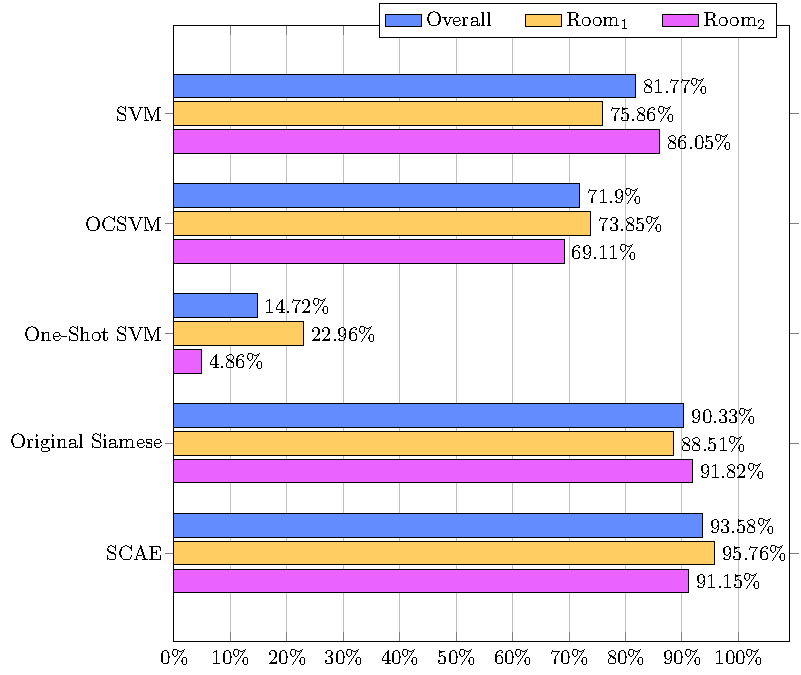
\includegraphics[width=\textwidth]{img/eeai/results_f1/results_f1}
	\caption[]
	{Results.} 
	\label{fig:results}
\end{figure*}
In \tableref{tab:cm_prai} and \tableref{tab:cm_scae} the normalized confusion matrix for the Siamese based approach are reported. As can be seen, the miss rate of the proposed method is less than 4\% compared to the \textit{Original Siamese} method, without losing in term of false alarm rate that, instead, has increased by 1\%, resulting in good improvements regarding the reliability of the system. Since there are many instances of background noise in the dataset, the low number of false alarms indicates that this approach could also be used as a detection system.

\begin{table}[t]
	\caption{Normalized confusion matrix of the \textit{Original Siamese} approach. Absolute values are shown in brackets.}
	\label{tab:cm_prai}
	\begin{center}
		\begin{tabular}[t]{C{3cm}|C{3cm}|C{3cm}}	
			
			\hline
			\textbf{\%} & \textbf{$\,$ Human Falls $\,$ } & \textbf{Objects} \\ %\cline{2-5} 
			\hline
			\textbf{$\,$ Human Falls $\,$ }     			& 90 (6283)    &  10 (690)     \\
			\textbf{Objects} 								& 9 (37)   &   91 (353)     	\\
			\hline
		\end{tabular}
	\end{center}
\end{table}
\begin{table}[t]
	\caption{Normalized confusion matrix of the SCAE approach. Absolute values are shown in brackets.}
	\label{tab:cm_scae}
	\begin{center}
		
		\begin{tabular}[t]{C{3cm}|C{3cm}|C{3cm}}
			\hline
			\textbf{\%}                                                    & \textbf{$\,$ Human Falls $\,$ } & \textbf{Objects} \\
			%\cline{2-5} 
			
			\hline
			\textbf{$\,$ Human Falls $\,$ } & 91 (6362)                       & 9 (611)          \\
			\textbf{Objects}                                               & 4 (17)                          & 96 (373)         \\ \hline
		\end{tabular}
	\end{center}
\end{table}

\section{Remarks}
In this work, previous work by the authors \cite{droghini2018fewshot} has been extended. First, a complete data set has been collected starting from the one used in the previous work. The recordings of A3Fall-v1.0 dataset have been extended with new events recorded in different environments and with different flooring. Moreover, in order to test the system, the dataset was augmented with 80 human falls performed by four actors. In this article, the authors have shown that the proposed method outperforms the other four comparative methods and that the same algorithm may be used not only as a classifier but also as a detector. In this more realistic scenario, the preeminence on the Siamese framework for one-shot learning with respect to conventional methods has been shown. A further improvement in performance has been achieved with an extension of the method previously proposed in \cite{droghini2018fewshot}. It is composed of 3 stages: log-mel feature extraction, metric learning employing a Siamese autoencoder neural network named SCAE and, in the end, a final decision stage base on \textit{knn} classifier. The network exploits the few information on the real fall by using a particular strategy of pairs generation for the SCAE training. In doing so, the system learns how to transform the available simulated human fall instances to create a more suitable set of templates that can be used to train the final classifier. 
%we think that this system may be employed as starting point from a company for a real application. During the installation in a company only need to performs some acquisition of every-day object falls, background noises and just one human fall performed by an actor to fine tune the model for a particular ambient. The rest of the dataset can be collected in laboratory with the aid of a manikin to simulate different fall patterns. ...
Although the system seems to be reliable because of the low miss rate, the false alarm rate, of just about 3 false alarms raised every 2 real human falls, may even so be annoying for some users. To reduce this problem, several techniques could be employed. For instance, the system could be extended to include algorithms for fall recovery recognition able to detect whether a person is continuing his normal activity or if he/she is still lying in the ground.
